% Options for packages loaded elsewhere
\PassOptionsToPackage{unicode}{hyperref}
\PassOptionsToPackage{hyphens}{url}
\PassOptionsToPackage{dvipsnames,svgnames,x11names}{xcolor}
%
\documentclass[
  10pt,
]{article}
\usepackage{amsmath,amssymb}
\usepackage{iftex}
\ifPDFTeX
  \usepackage[T1]{fontenc}
  \usepackage[utf8]{inputenc}
  \usepackage{textcomp} % provide euro and other symbols
\else % if luatex or xetex
  \usepackage{unicode-math} % this also loads fontspec
  \defaultfontfeatures{Scale=MatchLowercase}
  \defaultfontfeatures[\rmfamily]{Ligatures=TeX,Scale=1}
\fi
\usepackage{lmodern}
\ifPDFTeX\else
  % xetex/luatex font selection
\fi
% Use upquote if available, for straight quotes in verbatim environments
\IfFileExists{upquote.sty}{\usepackage{upquote}}{}
\IfFileExists{microtype.sty}{% use microtype if available
  \usepackage[]{microtype}
  \UseMicrotypeSet[protrusion]{basicmath} % disable protrusion for tt fonts
}{}
\makeatletter
\@ifundefined{KOMAClassName}{% if non-KOMA class
  \IfFileExists{parskip.sty}{%
    \usepackage{parskip}
  }{% else
    \setlength{\parindent}{0pt}
    \setlength{\parskip}{6pt plus 2pt minus 1pt}}
}{% if KOMA class
  \KOMAoptions{parskip=half}}
\makeatother
\usepackage{xcolor}
\usepackage[left=2cm, right=2cm, top=2cm, bottom=3cm, footskip = .5cm]{geometry}
\usepackage{longtable,booktabs,array}
\usepackage{calc} % for calculating minipage widths
% Correct order of tables after \paragraph or \subparagraph
\usepackage{etoolbox}
\makeatletter
\patchcmd\longtable{\par}{\if@noskipsec\mbox{}\fi\par}{}{}
\makeatother
% Allow footnotes in longtable head/foot
\IfFileExists{footnotehyper.sty}{\usepackage{footnotehyper}}{\usepackage{footnote}}
\makesavenoteenv{longtable}
\usepackage{graphicx}
\makeatletter
\def\maxwidth{\ifdim\Gin@nat@width>\linewidth\linewidth\else\Gin@nat@width\fi}
\def\maxheight{\ifdim\Gin@nat@height>\textheight\textheight\else\Gin@nat@height\fi}
\makeatother
% Scale images if necessary, so that they will not overflow the page
% margins by default, and it is still possible to overwrite the defaults
% using explicit options in \includegraphics[width, height, ...]{}
\setkeys{Gin}{width=\maxwidth,height=\maxheight,keepaspectratio}
% Set default figure placement to htbp
\makeatletter
\def\fps@figure{htbp}
\makeatother
\setlength{\emergencystretch}{3em} % prevent overfull lines
\providecommand{\tightlist}{%
  \setlength{\itemsep}{0pt}\setlength{\parskip}{0pt}}
\setcounter{secnumdepth}{-\maxdimen} % remove section numbering
% Set up the fonts
\usepackage[urw-palatino]{mathdesign}
\usepackage[T1]{fontenc}

% Add accessibility support from http://www.richschwinn.com/accessibility
\RequirePackage{accsupp}
\RequirePackage{pdfcomment}
\newcommand{\AccTool}[2]{\BeginAccSupp{method=pdfstringdef,unicode,Alt={{#1}}}\pdftooltip{{#2}}{{#1}}\EndAccSupp{}}

% Set the language for 508
\hypersetup{
  pdftitle = {title},
  pdflang = en-US}


% Set up the headers and footers
\usepackage{graphicx}
\usepackage{fancyhdr}
\usepackage{ifthen}
%\usepackage{everypage-1x}
\usepackage{float}
%\usepackage{subfig}
%\usepackage{subcaption}

% Avoid struggling over figure and table float in Rmarkdown
\let\origfigure\figure
\let\endorigfigure\endfigure
\renewenvironment{figure}[1][2] {
    \expandafter\origfigure\expandafter[H]
} {
    \endorigfigure
}

\let\origtable\table
\let\endorigtable\endtable
\renewenvironment{table}[1][2] {
    \expandafter\origtable\expandafter[H]
} {
    \endorigtable
}

% First page has the large title and NOAA logo
\pagestyle{fancy}
\fancyhf{}
\setlength\headheight{40pt}
\fancyheadoffset[L]{0.5cm}
\cfoot{\thepage}

\fancyheadinit{%
   \ifthenelse{\value{page}=4}%
      {\fancyhead[R]{
\includegraphics[width=40pt]{images/NOAA_logo.png} \\ \textsf{\emph{March 11, 2024}}}
       \fancyhead[L]{\textsf{\LARGE DRAFT State of the Ecosystem 2024: Mid-Atlantic}}
      }%
      {\fancyhead[R]{}
       \fancyhead[L]{\textsf{\emph{DRAFT State of the Ecosystem 2024: Mid-Atlantic}}}
      }
}



\renewcommand{\headrulewidth}{0.4pt}
\renewcommand{\footrulewidth}{0pt}

% Make caption fonts a bit smaller
\usepackage[font={small}]{caption}


% Change section labels to san serif
\usepackage{sectsty}
\allsectionsfont{\normalfont\sffamily\bfseries}
\usepackage{multirow}
\usepackage{multicol}
\usepackage{colortbl}
\usepackage{hhline}
\newlength\Oldarrayrulewidth
\newlength\Oldtabcolsep
\usepackage{longtable}
\usepackage{array}
\usepackage{hyperref}
\usepackage{float}
\usepackage{wrapfig}
\ifLuaTeX
  \usepackage{selnolig}  % disable illegal ligatures
\fi
\IfFileExists{bookmark.sty}{\usepackage{bookmark}}{\usepackage{hyperref}}
\IfFileExists{xurl.sty}{\usepackage{xurl}}{} % add URL line breaks if available
\urlstyle{same}
\hypersetup{
  colorlinks=true,
  linkcolor={Maroon},
  filecolor={Maroon},
  citecolor={Blue},
  urlcolor={blue},
  pdfcreator={LaTeX via pandoc}}

\author{}
\date{\vspace{-2.5em}}

\begin{document}

\setcounter{page}{4}
\thispagestyle{fancy}

\hypertarget{introduction}{%
\section{Introduction}\label{introduction}}

\hypertarget{about-this-report}{%
\subsection{About This Report}\label{about-this-report}}

This report is for the Mid-Atlantic Fishery Management Council (MAFMC). The purpose of this report is to synthesize ecosystem information to allow the MAFMC to better meet fishery management objectives, and to update the MAFMC's Ecosystem Approach to Fishery Management (EAFM) risk assessment. The major messages of the report are synthesized on pages 1 and 2, with highlights of 2023 ecosystem events on page 3. The information in this report is organized into two main sections; \protect\hyperlink{performance-relative-to-fishery-management-objectives}{performance measured against ecosystem-level management objectives} (Table \ref{tab:management-objectives}), and potential \protect\hyperlink{risks-to-meeting-fishery-management-objectives}{risks to meeting fishery management objectives} (\protect\hyperlink{climate-and-ecosystem-change}{climate change} and \protect\hyperlink{other-ocean-uses-offshore-wind}{other ocean uses}). A final new section introduced this year highlights \protect\hyperlink{highlights}{notable 2023 ecosystem observations}.

\hypertarget{report-structure}{%
\subsection{Report structure}\label{report-structure}}

The two main sections contain subsections for each management objective or potential risk. Within each subsection, we first review observed trends for indicators representing each objective or risk, including the status of the most recent data year relative to a threshold (if available) or relative to the long-term average. Second, we identify potential drivers of observed trends, and synthesize results of indicators related to those drivers to outline potential implications for management. For example, if there are multiple drivers related to an indicator trend, do indicators associated with the drivers have similar trends, and can any drivers be affected by management action(s)? We emphasize that these implications are intended to represent testable hypotheses at present, rather than ``answers,'' because the science behind these indicators and syntheses continues to develop.

A glossary of terms\footnote{\url{https://noaa-edab.github.io/tech-doc/glossary.html}}, detailed technical methods documentation\footnote{\url{https://NOAA-EDAB.github.io/tech-doc}}, indicator data\footnote{\url{https://noaa-edab.github.io/ecodata/}}, and detailed indicator descriptions\footnote{\url{https://noaa-edab.github.io/catalog/index.html}} are available online. We recommend new readers first review the details of standard figure formatting (Fig. \ref{fig:docformat}a), categorization of fish and invertebrate species into feeding guilds (Table \ref{tab:species-groupings}), and definitions of ecological production units (EPUs, including the Mid-Atlantic Bight, MAB; Fig. \ref{fig:docformat}b) provided at the end of the document.

\global\setlength{\Oldarrayrulewidth}{\arrayrulewidth}

\global\setlength{\Oldtabcolsep}{\tabcolsep}

\setlength{\tabcolsep}{0pt}

\renewcommand*{\arraystretch}{1}



\providecommand{\ascline}[3]{\noalign{\global\arrayrulewidth #1}\arrayrulecolor[HTML]{#2}\cline{#3}}

\begin{longtable}[c]{|p{1.42in}|p{4.09in}}

\caption{Ecosystem-scale\ fishery\ management\ objectives\ in\ the\ Mid-Atlantic\ Bight}\label{tab:management-objectives}\\

\ascline{1.5pt}{666666}{1-2}

\multicolumn{1}{>{\raggedright}m{\dimexpr 1.42in+0\tabcolsep}}{\textcolor[HTML]{000000}{\fontsize{9}{9}\selectfont{Objective\ categories}}} & \multicolumn{1}{>{\raggedright}m{\dimexpr 4.09in+0\tabcolsep}}{\textcolor[HTML]{000000}{\fontsize{9}{9}\selectfont{Indicators\ reported}}} \\

\ascline{1.5pt}{666666}{1-2}\endfirsthead \caption[]{Ecosystem-scale\ fishery\ management\ objectives\ in\ the\ Mid-Atlantic\ Bight}\label{tab:management-objectives}\\

\ascline{1.5pt}{666666}{1-2}

\multicolumn{1}{>{\raggedright}m{\dimexpr 1.42in+0\tabcolsep}}{\textcolor[HTML]{000000}{\fontsize{9}{9}\selectfont{Objective\ categories}}} & \multicolumn{1}{>{\raggedright}m{\dimexpr 4.09in+0\tabcolsep}}{\textcolor[HTML]{000000}{\fontsize{9}{9}\selectfont{Indicators\ reported}}} \\

\ascline{1.5pt}{666666}{1-2}\endhead



\multicolumn{2}{>{\raggedright}m{\dimexpr 5.51in+2\tabcolsep}}{\textcolor[HTML]{000000}{\fontsize{9}{9}\selectfont{\textbf{Provisioning\ and\ Cultural\ Services}}}} \\





\multicolumn{1}{>{\raggedright}m{\dimexpr 1.42in+0\tabcolsep}}{\textcolor[HTML]{000000}{\fontsize{9}{9}\selectfont{Seafood\ Production}}} & \multicolumn{1}{>{\raggedright}m{\dimexpr 4.09in+0\tabcolsep}}{\textcolor[HTML]{000000}{\fontsize{9}{9}\selectfont{Landings;\ commercial\ total\ and\ by\ feeding\ guild;\ recreational\ harvest}}} \\





\multicolumn{1}{>{\raggedright}m{\dimexpr 1.42in+0\tabcolsep}}{\textcolor[HTML]{000000}{\fontsize{9}{9}\selectfont{Profits}}} & \multicolumn{1}{>{\raggedright}m{\dimexpr 4.09in+0\tabcolsep}}{\textcolor[HTML]{000000}{\fontsize{9}{9}\selectfont{Revenue\ decomposed\ to\ price\ and\ volume}}} \\





\multicolumn{1}{>{\raggedright}m{\dimexpr 1.42in+0\tabcolsep}}{\textcolor[HTML]{000000}{\fontsize{9}{9}\selectfont{Recreation}}} & \multicolumn{1}{>{\raggedright}m{\dimexpr 4.09in+0\tabcolsep}}{\textcolor[HTML]{000000}{\fontsize{9}{9}\selectfont{Angler\ trips;\ recreational\ fleet\ diversity}}} \\





\multicolumn{1}{>{\raggedright}m{\dimexpr 1.42in+0\tabcolsep}}{\textcolor[HTML]{000000}{\fontsize{9}{9}\selectfont{Stability}}} & \multicolumn{1}{>{\raggedright}m{\dimexpr 4.09in+0\tabcolsep}}{\textcolor[HTML]{000000}{\fontsize{9}{9}\selectfont{Diversity\ indices\ (fishery\ and\ ecosystem)}}} \\





\multicolumn{1}{>{\raggedright}m{\dimexpr 1.42in+0\tabcolsep}}{\textcolor[HTML]{000000}{\fontsize{9}{9}\selectfont{Social\ \&\ Cultural}}} & \multicolumn{1}{>{\raggedright}m{\dimexpr 4.09in+0\tabcolsep}}{\textcolor[HTML]{000000}{\fontsize{9}{9}\selectfont{Community\ engagement/reliance\ and\ environmental\ justice\ status}}} \\





\multicolumn{1}{>{\raggedright}m{\dimexpr 1.42in+0\tabcolsep}}{\textcolor[HTML]{000000}{\fontsize{9}{9}\selectfont{Protected\ Species}}} & \multicolumn{1}{>{\raggedright}m{\dimexpr 4.09in+0\tabcolsep}}{\textcolor[HTML]{000000}{\fontsize{9}{9}\selectfont{Bycatch;\ population\ (adult\ and\ juvenile)\ numbers;\ mortalities}}} \\





\multicolumn{2}{>{\raggedright}m{\dimexpr 5.51in+2\tabcolsep}}{\textcolor[HTML]{000000}{\fontsize{9}{9}\selectfont{\textbf{Supporting\ and\ Regulating\ Services}}}} \\





\multicolumn{1}{>{\raggedright}m{\dimexpr 1.42in+0\tabcolsep}}{\textcolor[HTML]{000000}{\fontsize{9}{9}\selectfont{Biomass}}} & \multicolumn{1}{>{\raggedright}m{\dimexpr 4.09in+0\tabcolsep}}{\textcolor[HTML]{000000}{\fontsize{9}{9}\selectfont{Biomass\ or\ abundance\ by\ feeding\ guild\ from\ surveys}}} \\





\multicolumn{1}{>{\raggedright}m{\dimexpr 1.42in+0\tabcolsep}}{\textcolor[HTML]{000000}{\fontsize{9}{9}\selectfont{Productivity}}} & \multicolumn{1}{>{\raggedright}m{\dimexpr 4.09in+0\tabcolsep}}{\textcolor[HTML]{000000}{\fontsize{9}{9}\selectfont{Condition\ and\ recruitment\ of\ managed\ species,\ primary\ productivity}}} \\





\multicolumn{1}{>{\raggedright}m{\dimexpr 1.42in+0\tabcolsep}}{\textcolor[HTML]{000000}{\fontsize{9}{9}\selectfont{Trophic\ structure}}} & \multicolumn{1}{>{\raggedright}m{\dimexpr 4.09in+0\tabcolsep}}{\textcolor[HTML]{000000}{\fontsize{9}{9}\selectfont{Relative\ biomass\ of\ feeding\ guilds,\ zooplankton}}} \\





\multicolumn{1}{>{\raggedright}m{\dimexpr 1.42in+0\tabcolsep}}{\textcolor[HTML]{000000}{\fontsize{9}{9}\selectfont{Habitat}}} & \multicolumn{1}{>{\raggedright}m{\dimexpr 4.09in+0\tabcolsep}}{\textcolor[HTML]{000000}{\fontsize{9}{9}\selectfont{Estuarine\ and\ offshore\ habitat\ conditions}}} \\

\ascline{1.5pt}{666666}{1-2}



\end{longtable}



\arrayrulecolor[HTML]{000000}

\global\setlength{\arrayrulewidth}{\Oldarrayrulewidth}

\global\setlength{\tabcolsep}{\Oldtabcolsep}

\renewcommand*{\arraystretch}{1}

\hypertarget{performance-relative-to-fishery-management-objectives}{%
\section{Performance Relative to Fishery Management Objectives}\label{performance-relative-to-fishery-management-objectives}}

In this section, we examine indicators related to broad, ecosystem-level fishery management objectives. We also provide hypotheses on the implications of these trends---why we are seeing them, what's driving them, and potential or observed regime shifts or changes in ecosystem structure. Identifying multiple drivers, regime shifts, and potential changes to ecosystem structure, as well as identifying the most vulnerable resources, can help managers determine whether anything needs to be done differently to meet objectives and how to prioritize upcoming issues/risks.

\hypertarget{seafood-production}{%
\subsection{Seafood Production}\label{seafood-production}}

\hypertarget{indicators-landings-commercial-and-recreational}{%
\subsubsection{Indicators: Landings; commercial and recreational}\label{indicators-landings-commercial-and-recreational}}

This year, we present updated indicators for total \href{https://noaa-edab.github.io/catalog/comdat.html}{commercial landings}, U.S. seafood landings, and Council-managed U.S. seafood landings. Total commercial landings within the Mid-Atlantic have declined over the long term, and total U.S. Mid-Atlantic seafood landings are near their all time low. Because there is no long term trend in MAFMC-managed U.S. seafood landings, the decline in U.S. seafood landings in the Mid-Atlantic region is likely driven by recent declines in species not managed by the Mid-Atlantic Council (Fig. \ref{fig:total-landings}).

\begin{figure}

{\centering \includegraphics{SOE-MAFMC-2024_files/figure-latex/total-landings-1} 

}

\caption{Total commercial landings (black), total U.S. seafood landings (blue), and Mid-Atlantic managed U.S. seafood landings (red), with significant declines (purple) in total and U.S. seafood landings.}\label{fig:total-landings}
\end{figure}

Commercial landings by guild include all species and all uses, and are reported as total for the guild and the MAFMC managed species within the \href{https://noaa-edab.github.io/catalog/species_groupings.html}{guild}. As reported in previous years, landings of benthos presented a significant downward trend, primarily driven by surf clam and ocean quahog, with scallops now contributing to the decline as well. However, total landings of planktivores is now also presenting a significant downward trend, primarily due to decreases in species not managed by the MAFMC (Atlantic herring and Atlantic menhaden; Fig. \ref{fig:comm-landings}).

\begin{figure}

{\centering \includegraphics{SOE-MAFMC-2024_files/figure-latex/comm-landings-1} 

}

\caption{Total commercial landings in the Mid-Atlantic Bight (black) and MAFMC-managed U.S seafood landings (red) by feeding guild, with significant declines (purple) in total planktivore landings and both total and MAFMC managed benthos landings and a significant increase (orange) in total benthivore landings.}\label{fig:comm-landings}
\end{figure}

\begin{verbatim}
## Error in nlme::gls(y ~ x + x2, data = data, correlation = nlme::corAR1(form = ~x),  : 
##   false convergence (8)
\end{verbatim}

Although total \href{https://noaa-edab.github.io/catalog/recdat.html}{recreational harvest} (retained fish presumed to be eaten) has increased from a historic low in 2018, there is a long-term decline in the MAB (Fig. \ref{fig:rec-landings}).

\begin{figure}

{\centering \includegraphics{SOE-MAFMC-2024_files/figure-latex/rec-landings-1} 

}

\caption{Total recreational seafood harvest (millions of pounds, black, significant decrease, purple) in the Mid-Atlantic region.}\label{fig:rec-landings}
\end{figure}

\href{https://noaa-edab.github.io/catalog/rec_hms.html}{Recreational shark landings} show an increase in pelagic sharks over the past decade, with a sharp decrease in 2018 - 2019 persisting through 2022 (Fig \ref{fig:rec-hms}). This is likely influenced by regulatory changes implemented in 2018 intended to rebuild shortfin mako stocks.

\begin{figure}

{\centering \includegraphics{SOE-MAFMC-2024_files/figure-latex/rec-hms-1} 

}

\caption{Recreational shark landings from Large Pelagics Survey.}\label{fig:rec-hms}
\end{figure}

Aquaculture production is not yet included in total seafood landings. Available \href{https://noaa-edab.github.io/catalog/aquaculture.html}{aquaculture production} of oysters for a subset of Mid-Atlantic states indicates a decline in recent years.

\hypertarget{implications}{%
\subsubsection{Implications}\label{implications}}

Declining commercial (total and seafood) and recreational landings can be driven by many interacting factors, including combinations of ecosystem and stock production, management actions, market conditions, and environmental change. While we cannot evaluate all possible drivers at present, here we evaluate the extent to which stock status and system biomass trends may play a role.

\hypertarget{stock-status-and-catch-limits}{%
\paragraph{Stock Status and Catch Limits}\label{stock-status-and-catch-limits}}

Single species \href{https://noaa-edab.github.io/catalog/stock_status.html}{management objectives} (1. maintaining biomass above minimum thresholds and 2. maintaining fishing mortality below overfishing limits) are being met for all but two MAFMC-managed species (Fig. \ref{fig:stock-status}), though the status of six stocks is unknown (Table \ref{tab:unkstocks}).

\begin{figure}

{\centering \includegraphics{SOE-MAFMC-2024_files/figure-latex/stock-status-1} 

}

\caption{Summary of single species status for MAFMC and jointly federally managed stocks (Spiny dogfish and both Goosefish). The dotted vertical line is the target biomass reference point of $B_{MSY}$. The dashed lines are the management thresholds of one half $B_{MSY}$ (vertical) or $F_{MSY}$. (horizontal). Stocks in orange are below the biomass threshold (overfished) or have fishing mortality above the limit (subject to overfishing), so are not meeting objectives. Stocks in purple  are above the biomass threshold but below the biomass target with fishing mortality within the limit. Stocks in green are above the biomass target, with fishing mortality within the limit.}\label{fig:stock-status}
\end{figure}

\global\setlength{\Oldarrayrulewidth}{\arrayrulewidth}

\global\setlength{\Oldtabcolsep}{\tabcolsep}

\setlength{\tabcolsep}{0pt}

\renewcommand*{\arraystretch}{1.5}



\providecommand{\ascline}[3]{\noalign{\global\arrayrulewidth #1}\arrayrulecolor[HTML]{#2}\cline{#3}}

\begin{longtable}[c]{|p{3.29in}|p{0.70in}|p{0.72in}}

\caption{Unknown\ or\ partially\ known\ stock\ status\ for\ MAFMC\ and\ jointly\ managed\ species.}\label{tab:unkstocks}\\

\ascline{1.5pt}{666666}{1-3}

\multicolumn{1}{>{\raggedright}m{\dimexpr 3.29in+0\tabcolsep}}{\textcolor[HTML]{000000}{\fontsize{9}{9}\selectfont{Stock}}} & \multicolumn{1}{>{\raggedleft}m{\dimexpr 0.7in+0\tabcolsep}}{\textcolor[HTML]{000000}{\fontsize{9}{9}\selectfont{F/Fmsy}}} & \multicolumn{1}{>{\raggedleft}m{\dimexpr 0.72in+0\tabcolsep}}{\textcolor[HTML]{000000}{\fontsize{9}{9}\selectfont{B/Bmsy}}} \\

\ascline{1.5pt}{666666}{1-3}\endfirsthead \caption[]{Unknown\ or\ partially\ known\ stock\ status\ for\ MAFMC\ and\ jointly\ managed\ species.}\label{tab:unkstocks}\\

\ascline{1.5pt}{666666}{1-3}

\multicolumn{1}{>{\raggedright}m{\dimexpr 3.29in+0\tabcolsep}}{\textcolor[HTML]{000000}{\fontsize{9}{9}\selectfont{Stock}}} & \multicolumn{1}{>{\raggedleft}m{\dimexpr 0.7in+0\tabcolsep}}{\textcolor[HTML]{000000}{\fontsize{9}{9}\selectfont{F/Fmsy}}} & \multicolumn{1}{>{\raggedleft}m{\dimexpr 0.72in+0\tabcolsep}}{\textcolor[HTML]{000000}{\fontsize{9}{9}\selectfont{B/Bmsy}}} \\

\ascline{1.5pt}{666666}{1-3}\endhead



\multicolumn{1}{>{\raggedright}m{\dimexpr 3.29in+0\tabcolsep}}{\textcolor[HTML]{000000}{\fontsize{9}{9}\selectfont{Longfin\ inshore\ squid\ -\ Georges\ Bank\ /\ Cape\ Hatteras}}} & \multicolumn{1}{>{\raggedleft}m{\dimexpr 0.7in+0\tabcolsep}}{\textcolor[HTML]{000000}{\fontsize{9}{9}\selectfont{-}}} & \multicolumn{1}{>{\raggedleft}m{\dimexpr 0.72in+0\tabcolsep}}{\textcolor[HTML]{000000}{\fontsize{9}{9}\selectfont{2.873}}} \\





\multicolumn{1}{>{\raggedright}m{\dimexpr 3.29in+0\tabcolsep}}{\textcolor[HTML]{000000}{\fontsize{9}{9}\selectfont{Northern\ shortfin\ squid\ -\ Northwestern\ Atlantic\ Coast}}} & \multicolumn{1}{>{\raggedleft}m{\dimexpr 0.7in+0\tabcolsep}}{\textcolor[HTML]{000000}{\fontsize{9}{9}\selectfont{-}}} & \multicolumn{1}{>{\raggedleft}m{\dimexpr 0.72in+0\tabcolsep}}{\textcolor[HTML]{000000}{\fontsize{9}{9}\selectfont{-}}} \\





\multicolumn{1}{>{\raggedright}m{\dimexpr 3.29in+0\tabcolsep}}{\textcolor[HTML]{000000}{\fontsize{9}{9}\selectfont{Goosefish\ -\ Gulf\ of\ Maine\ /\ Northern\ Georges\ Bank}}} & \multicolumn{1}{>{\raggedleft}m{\dimexpr 0.7in+0\tabcolsep}}{\textcolor[HTML]{000000}{\fontsize{9}{9}\selectfont{-}}} & \multicolumn{1}{>{\raggedleft}m{\dimexpr 0.72in+0\tabcolsep}}{\textcolor[HTML]{000000}{\fontsize{9}{9}\selectfont{-}}} \\





\multicolumn{1}{>{\raggedright}m{\dimexpr 3.29in+0\tabcolsep}}{\textcolor[HTML]{000000}{\fontsize{9}{9}\selectfont{Goosefish\ -\ Southern\ Georges\ Bank\ /\ Mid-Atlantic}}} & \multicolumn{1}{>{\raggedleft}m{\dimexpr 0.7in+0\tabcolsep}}{\textcolor[HTML]{000000}{\fontsize{9}{9}\selectfont{-}}} & \multicolumn{1}{>{\raggedleft}m{\dimexpr 0.72in+0\tabcolsep}}{\textcolor[HTML]{000000}{\fontsize{9}{9}\selectfont{-}}} \\

\ascline{1.5pt}{666666}{1-3}



\end{longtable}



\arrayrulecolor[HTML]{000000}

\global\setlength{\arrayrulewidth}{\Oldarrayrulewidth}

\global\setlength{\tabcolsep}{\Oldtabcolsep}

\renewcommand*{\arraystretch}{1}

Stock status affects catch limits established by the Council, which in turn may affect landings trends. Summed across all MAFMC managed species, total Acceptable Biological Catch or Annual Catch Limits \href{https://noaa-edab.github.io/catalog/abc_acl.html}{(ABC or ACL)} have been relatively stable 2012-2022 (Fig. \ref{fig:abcacl-stacked}). The recent total ABC or ACL is lower relative to 2012-2013, with much of that decrease due to declining Atlantic mackerel ABC. This is true even with the addition of blueline tilefish management in 2017 contributing an additional ABC and ACL to the total 2017-2022, due to that fishery's small relative size.

\begin{figure}

{\centering \includegraphics{SOE-MAFMC-2024_files/figure-latex/abcacl-stacked-1} 

}

\caption{Sum of catch limits across all MAFMC managed commercial (C) and recreational (R) fisheries.}\label{fig:abcacl-stacked}
\end{figure}

Nevertheless, the percentage caught (landings and discards) for each stock's ABC/ACL suggests that these catch limits are not generally constraining as most species are well below the 1/1 ratio (Fig. \ref{fig:abcacl-catch}). Therefore, stock status and associated management constraints are unlikely to be driving decreased landings for the majority of species.

\begin{figure}

{\centering \includegraphics{SOE-MAFMC-2024_files/figure-latex/abcacl-catch-1} 

}

\caption{Catch divided by ABC/ACL for MAFMC managed fisheries. High points are recreational black sea bass (up to 2021) and scup (2022). Red line indicates the median ratio across all fisheries.}\label{fig:abcacl-catch}
\end{figure}

\hypertarget{system-biomass}{%
\paragraph{System Biomass}\label{system-biomass}}

Although \href{https://noaa-edab.github.io/catalog/aggregate_biomass.html}{aggregate biomass} trends derived from scientific resource surveys are mostly stable in the MAB, spring piscivores and fall benthivores show long-term increases (Fig. \ref{fig:nefsc-biomass-mab}). While managed species make up varying proportions of aggregate biomass, trends in landings are not mirroring shifts in the overall trophic structure of survey-sampled fish and invertebrates. Therefore, major shifts in feeding guilds or ecosystem trophic structure are unlikely to be driving the decline in landings.

\begin{figure}

{\centering \includegraphics{SOE-MAFMC-2024_files/figure-latex/nefsc-biomass-mab-1} 

}

\caption{Spring (left) and fall (right) surveyed biomass in the Mid-Atlantic Bight. Data from the NEFSC Bottom Trawl Survey are shown in black, with the nearshore NEAMAP survey shown in red. Significant increases (orange lines) are present for spring piscivore and fall benthivore biomass. The shaded area around each annual mean represents 2 standard deviations from the mean.}\label{fig:nefsc-biomass-mab}
\end{figure}

\hypertarget{effect-on-seafood-production}{%
\paragraph{Effect on Seafood Production}\label{effect-on-seafood-production}}

Stock status is above the minimum threshold for all but two stocks, and aggregate biomass trends appear stable, so the decline in managed commercial seafood landings is most likely driven by market dynamics affecting the landings of surfclams and ocean quahogs, as landings have been below quotas for these species. In addition, regional availability of scallops has contributed to the decline of benthos landings not managed by the MAFMC, with some of the most productive grounds currently closed through rotational management. The long term decline in total planktivore landings is largely driven by Atlantic menhaden fishery dynamics, including a consolidation of processors leading to reduced fishing capacity between the 1990s and mid-2000s.

Climate change also seems to be shifting the distribution of surfclams and ocean quahogs, resulting in areas with overlapping distributions and increased mixed landings. Given the regulations governing mixed landings, this could become problematic in the future and is currently being evaluated by the Council.

The decline in recreational seafood harvest stems from other drivers. Some of the decline, such as that for recreational shark landings, is driven by management intended to reduce fishing mortality on mako sharks. However, NOAA Fisheries' Marine Recreational Information Program survey methodology was updated in 2018, so it is unclear whether the lower than average landings for species other than sharks since 2018 are driven by changes in fishing behavior or the change in the survey methodology. Nevertheless, the recreational harvest seems to be stabilizing at a lower level than historical estimates.

Other environmental changes require monitoring as they may become important drivers of landings in the future:

\begin{itemize}
\tightlist
\item
  Climate is trending into uncharted territory. Globally, 2023 was the warmest year on record (see \protect\hyperlink{highlights}{2023 Highlights section}).
\item
  Stocks are shifting their distributions, moving towards the northeast and into deeper waters throughout the Northeast US Large Marine Ecosystem (see \protect\hyperlink{climate-and-ecosystem-change}{Climate Risks section}).
\item
  Some ecosystem composition and production changes have been observed (see \protect\hyperlink{stability}{Stability section}).
\item
  Some fishing communities are affected by environmental justice vulnerabilities (see \protect\hyperlink{environmental-justice-and-social-vulnerability}{Environmental Justice and Social Vulnerability section}).
\end{itemize}

\hypertarget{commercial-profits}{%
\subsection{Commercial Profits}\label{commercial-profits}}

\hypertarget{indicators-revenue-a-proxy-for-profits}{%
\subsubsection{Indicators: revenue (a proxy for profits)}\label{indicators-revenue-a-proxy-for-profits}}

Total \href{https://noaa-edab.github.io/catalog/comdat.html}{commercial revenue} and MAFMC managed species revenue within the Mid-Atlantic Bight have declined over the past 20-30 years. In 2022, total revenue was at an all-time low, and revenue from MAFMC managed species was near an all-time low (Fig. \ref{fig:comm-revenue}).

\begin{figure}

{\centering \includegraphics{SOE-MAFMC-2024_files/figure-latex/comm-revenue-1} 

}

\caption{Revenue for the for the Mid-Atlantic region: total (black) and from MAFMC managed species (red), with a significant decrease (purple) for total revenue.}\label{fig:comm-revenue}
\end{figure}

Revenue earned by harvesting resources is a function of both the quantity landed of each species and the prices paid for landings. Beyond monitoring yearly changes in revenue, it is even more valuable to determine what drives these changes: harvest levels, the mix of species landed, price changes, or a combination of these. The \href{https://noaa-edab.github.io/catalog/bennet.html}{Bennet Indicator} decomposes revenue change into two parts, one driven by changing quantities (volumes), and a second driven by changing prices. All changes are in relation to a base year (1982).

In the Mid-Atlantic region revenues were above the 1982 baseline for all years in the series until 2022 (Fig. \ref{fig:bennet}). Both increasing prices and volumes contributed to the positive revenue change in most years. In terms of prices, since 2000 Benthos contributed the most to increasing prices (Fig. \ref{fig:bennet-all}). Beginning in the 1990s, in most years benthivores contributed the most to increasing volumes (Fig. \ref{fig:bennet-all}).

\begin{figure}

{\centering \includegraphics{SOE-MAFMC-2024_files/figure-latex/bennet-1} 

}

\caption{Revenue change from 1982 values in 2022 dollars (black); Price (PI), and Volume Indicators (VI) for total commercial landings in the Mid-Atlantic Bight.}\label{fig:bennet}
\end{figure}

\begin{figure}

{\centering \includegraphics{SOE-MAFMC-2024_files/figure-latex/bennet-all-1} 

}

\caption{Total price and volume indicators in 2022 dollars (black) for commercial landings, and individual guild contributions to each indicator, in the Mid-Atlantic Bight.}\label{fig:bennet-all}
\end{figure}

\hypertarget{implications-1}{%
\subsubsection{Implications}\label{implications-1}}

Although the Mid-Atlantic region shows declining revenue trends since 2016, inflation-adjusted revenue from harvested species was still greater than 1982 levels until 2022. In a similar manner to seafood landings, the results here are driven in large part by market dynamics affecting the landings of surfclams and ocean quahogs, as landings have been below quotas for these species, as well as lower quotas for Atlantic scallops. The declining Benthos category since 2012 may be partially caused by decreases in surfclam and ocean quahogs in the southern part of their range as harvest have shifted northward. Changes in other indicators, particularly those driving landings and those related to climate change, require monitoring as they may become important drivers of revenue in the future; for example:

\begin{itemize}
\tightlist
\item
  Surfclams, ocean quahogs, and scallops are sensitive to warming ocean temperatures and ocean acidification.\\
\item
  \href{https://noaa-edab.github.io/catalog/ocean_acidification}{Multiple stressors} are interacting in Mid-Atlantic shellfish habitats.
\end{itemize}

\hypertarget{recreational-opportunities}{%
\subsection{Recreational Opportunities}\label{recreational-opportunities}}

\hypertarget{indicators-angler-trips-fleet-diversity}{%
\subsubsection{Indicators: Angler trips, fleet diversity}\label{indicators-angler-trips-fleet-diversity}}

\href{https://noaa-edab.github.io/catalog/recdat.html}{Recreational effort} (angler trips) in 2022 has increased and is above the long-term average (Fig. \ref{fig:rec-op}). in the MAB. However, recreational fleet diversity (i.e., effort by shoreside, private boat, and for-hire anglers) has declined over the long term (Fig. \ref{fig:rec-div}).

\begin{figure}

{\centering \includegraphics{SOE-MAFMC-2024_files/figure-latex/rec-op-1} 

}

\caption{Recreational effort (number of trips, black) in the Mid-Atlantic, with significant increase (orange line).}\label{fig:rec-op}
\end{figure}

\begin{figure}

{\centering \includegraphics{SOE-MAFMC-2024_files/figure-latex/rec-div-1} 

}

\caption{Recreational fleet effort diversity (black) in the Mid-Atlantic, with significant decrease (purple line).}\label{fig:rec-div}
\end{figure}

\hypertarget{implications-2}{%
\subsubsection{Implications}\label{implications-2}}

While the overall number of recreational opportunities in the MAB is above the long-term average, the continuing decline in recreational fleet effort diversity suggests a potentially reduced range of recreational fishing options, despite the slight increase in this indicator's value between 2020 and 2022.

The downward effort diversity trend is driven by party/charter contraction (down from 2\% in 2021 to 1.4\% in 2023), and a shift toward shorebased angling, which currently makes up 59\% of angler trips. Effort in private boats has increased slightly to 40\% of trips from 37\% in 2021.

Changes in recreational fleet diversity can be considered when managers seek options to maintain recreational opportunities. Shore anglers will have access to different species than vessel-based anglers, and when the same species is accessible both from shore and from a vessel, shore anglers typically have access to smaller individuals. Many states have developed shore-based regulations where the minimum size is lower than in other areas and sectors to maintain opportunities in the shore angling sector.

\hypertarget{stability}{%
\subsection{Stability}\label{stability}}

\hypertarget{indicators-fishery-fleet-and-catch-diversity-ecological-component-diversity}{%
\subsubsection{Indicators: fishery fleet and catch diversity, ecological component diversity}\label{indicators-fishery-fleet-and-catch-diversity-ecological-component-diversity}}

While there are many potential metrics of stability, we use diversity indices to evaluate overall stability in fisheries and ecosystems. In general, diversity that remains constant over time suggests a similar capacity to respond to change over time. A significant change in diversity over time does not necessarily indicate a problem or an improvement, but does indicate a need for further investigation. We examine diversity in commercial fleet and species catch, recreational species catch (with fleet effort diversity discussed above), zooplankton, and adult fishes.

\hypertarget{fishery-stability}{%
\paragraph{Fishery Stability}\label{fishery-stability}}

\href{https://noaa-edab.github.io/catalog/commercial_div.html}{Diversity} estimates have been developed for fleets landing managed species, and species landed by commercial vessels with Mid-Atlantic permits. Commercial fishery fleet count and fleet diversity have been stable over time in the MAB, with current values near the long-term average. This indicates similar commercial fleet composition and species targeting opportunities over time. Commercial fisheries are relying on fewer species relative to the mid-90s, although current species revenue diversity has recovered somewhat in the last year (Fig. \ref{fig:commercial-div-species-div}).

\begin{figure}

{\centering \includegraphics{SOE-MAFMC-2024_files/figure-latex/commercial-div-species-div-1} 

}

\caption{Species revenue diversity in the Mid Atlantic.}\label{fig:commercial-div-species-div}
\end{figure}

As noted \protect\hyperlink{recreational-opportunities}{above}, \href{https://noaa-edab.github.io/catalog/recdat.html}{recreational fleet effort diversity} is declining (Fig. \ref{fig:rec-div}), suggesting a shift in recreational fishing opportunities. However, recreational species catch diversity has no long term trend so is considered stable, and has been at or above the long term average in 8 of the last 10 years (Fig. \ref{fig:recdat-div-catch}).

\begin{figure}

{\centering \includegraphics{SOE-MAFMC-2024_files/figure-latex/recdat-div-catch-1} 

}

\caption{Diversity of recreational catch in the Mid Atlantic.}\label{fig:recdat-div-catch}
\end{figure}

\hypertarget{ecological-stability}{%
\paragraph{Ecological Stability}\label{ecological-stability}}

Total \href{https://noaa-edab.github.io/catalog/chl_pp.html}{primary production} (PP) is a measure of the total energy input into a system per year. Total primary production in the Mid Atlantic has no clear trend (Fig. \ref{fig:totpp}), suggesting stability in energy at the base of the food web.

\begin{figure}

{\centering \includegraphics{SOE-MAFMC-2024_files/figure-latex/totpp-1} 

}

\caption{Total areal annual primary production for the MAB. The dashed line represents the long-term (1998-2023) annual mean.}\label{fig:totpp}
\end{figure}

Ecological diversity indices show mixed trends. \href{https://noaa-edab.github.io/catalog/zoo_diversity.html}{Zooplankton diversity} is increasing in the MAB (Fig. \ref{fig:zoo-diversity}). \href{https://noaa-edab.github.io/catalog/exp_n.html}{Adult fish diversity} is measured as the expected number of species in a standard number of individuals sampled from the NEFSC bottom trawl survey. Adult fish diversity indices appear stable over time, with current values within one standard deviation from most historic estimates (Fig. \ref{fig:exp-n}).

\begin{figure}

{\centering \includegraphics{SOE-MAFMC-2024_files/figure-latex/zoo-diversity-1} 

}

\caption{Zooplankton diversity in the Mid-Atlantic Bight, Shannon diversity index (black) with significant increase (orange line).}\label{fig:zoo-diversity}
\end{figure}

\begin{figure}

{\centering \includegraphics{SOE-MAFMC-2024_files/figure-latex/exp-n-1} 

}

\caption{Adult fish diversity in the Mid-Atlantic Bight, based on expected number of species. Results from survey vessels Albatross and Bigelow are reported separately due to catchability differences.}\label{fig:exp-n}
\end{figure}

\hypertarget{implications-3}{%
\subsubsection{Implications}\label{implications-3}}

Fleet diversity indices are used by the MAFMC to evaluate stability objectives as well as risks to fishery resilience and maintaining equity in access to fishery resources. Stability in commercial fleet diversity metrics suggests stable capacity to respond to the current range of fishing opportunities. However, commercial species diversity remains low when compared to historical levels.

Declining recreational fleet effort diversity, as noted above, indicates that the party/charter boat sector continues to contract, with shoreside angling becoming more important as a percentage of recreational angler trips. Stability in recreational species catch diversity has been maintained by a different set of species over time. A recent increase in Atlantic States Marine Fisheries Commission (ASMFC) and South Atlantic Fishery Management Council (SAFMC) managed species in recreational catch is helping to maintain diversity in the same range that MAFMC and New England Fishery Management Council (NEFMC) managed species supported in the 1990s.

Production at the base of the food web is variable, but stable over time. Ecological diversity indices can provide insight into ecosystem structure. Changes in ecological diversity over time may indicate altered ecosystem structure with implications for fishery productivity and management. Stable adult fish diversity indicates the same overall number and evenness over time, but doesn't rule out species substitutions (e.g., warm-water replacing cold-water). In addition, the change in survey vessels complicates interpretation of long-term fish diversity trends.

In the MAB, existing diversity indicators suggest overall stability in the fisheries and ecosystem components examined. However, declining recreational fleet diversity suggests a potential loss in the range of recreational fishing opportunities. Increasing zooplankton diversity (due to increases in abundance of several taxa and stable or declining dominance of an important copepod species) suggests a shift in the zooplankton community that warrants continued monitoring to determine if managed species are affected. In addition, the species diversity in commercial landings warrants continued attention given its relatively low index value indicating average reliance on a small number of species for revenue.

\hypertarget{environmental-justice-and-social-vulnerability}{%
\subsection{Environmental Justice and Social Vulnerability}\label{environmental-justice-and-social-vulnerability}}

Providing for sustained participation of fishing communities, and avoiding adverse economic impacts to fishing communities are objectives of fishery management. We report the top ten communities most engaged in, and/or reliant upon, commercial and recreational fisheries and the degree to which these communities may be vulnerable to environmental justice issues (i.e., Poverty, Population Composition, and Personal Disruption) using data for the most recent available year (2021). We also compare these results with those presented in previous SOE reports to highlight changes in community status.

\hypertarget{indicators-environmental-justice-and-social-vulnerability-in-commercial-and-recreational-fishing-communities}{%
\subsubsection{Indicators: Environmental Justice and Social Vulnerability in commercial and recreational fishing communities}\label{indicators-environmental-justice-and-social-vulnerability-in-commercial-and-recreational-fishing-communities}}

The \href{https://noaa-edab.github.io/catalog/engagement.html}{engagement and reliance} indices demonstrate the importance of commercial and recreational fishing to a given community relative to other coastal communities in a region. Social vulnerability indicators measure social factors that shape a community's ability to adapt to change. A subset of these factors can be used to assess potential environmental justice issues. Similarly to the engagement and reliance indicators, the environmental justice indices characterize different facets and levels of social vulnerability in a given community relative to other coastal communities in a region.

Changes in fishing activity between years changed community engagement and reliance rankings. The largest change from last year's report is that Hatteras and Hobucken, NC are no longer listed as top ten commercial fishing communities, replaced by Hampton, VA; Swan Quarter, NC; Bowers and Little Creek, DE (Fig.\ref{fig:commercial-engagement}). Manteo, Vandemere, and Hobuken, NC are no longer listed as top ten recreational communities, replaced by Cape May and Barnegat Light, NJ; Orient, NY; Topsail Beach, Avon and Rodanthe, NC (Fig.\ref{fig:recreational-engagement}).

\begin{figure}

{\centering \includegraphics{SOE-MAFMC-2024_files/figure-latex/commercial-engagement-1} 

}

\caption{Commercial engagement, reliance, and environmental justice vulnerability for the top commercially engaged and reliant fishing communities in the Mid-Atlantic.}\label{fig:commercial-engagement}
\end{figure}

Scores for environmental justice concerns remain similar for communities based on 2020 and 2021 data, with top commercial ports (Fig. \ref{fig:commercial-EJ}) showing more concerns than top recreational ports overall (Fig. \ref{fig:recreational-EJ}). Atlantic City, NJ ranks highest for all three environmental justice concerns. There is variability in the specific issues facing communities with environmental justice concerns. Higher scores in population composition indicate community vulnerability related to the presence of non-white, non-English speaking, and younger populations.

\begin{figure}

{\centering \includegraphics{SOE-MAFMC-2024_files/figure-latex/recreational-engagement-1} 

}

\caption{Recreational engagement and reliance, and environmental justice vulnerability, for the top recreationally engaged and reliant fishing communities in the Mid-Atlantic.}\label{fig:recreational-engagement}
\end{figure}

Both commercial and recreational fishing are important activities in Montauk, NY, Cape May, Barnegat Light and Point Pleasant Beach, NJ; and Rodanthe, NC, meaning these communities may be impacted simultaneously by commercial and recreational regulatory changes. However, in all but Point Pleasant Beach NJ, environmental justice may not be a major concern in these communities given the index scores (Figs \ref{fig:commercial-EJ} and \ref{fig:recreational-EJ})). Point Pleasant Beach, NJ scored medium for the personal disruption index, indicating that environmental justice may be a moderate concern in Point Pleasant Beach.

\begin{figure}

{\centering 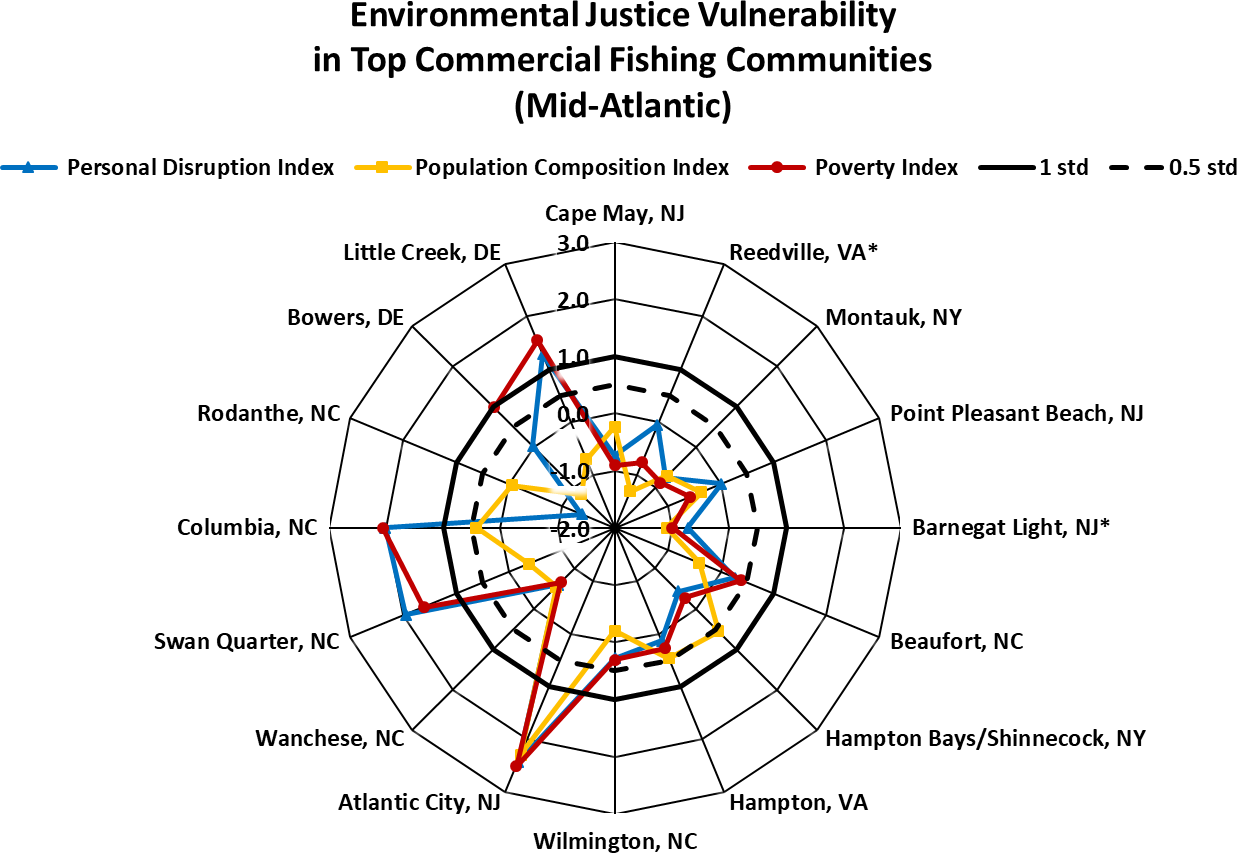
\includegraphics[width=0.75\linewidth]{SOE-MAFMC-2024_files/figure-latex/commercial-EJ-1} 

}

\caption{Environmental justice indicators (Poverty Index, population composition index, and personal disruption index) for top commercial fishing communities in Mid-Atlantic. Some communities are missing data for some indices. *Community scored high (1.00 and above) for both commercial engagement and reliance indicators.}\label{fig:commercial-EJ}
\end{figure}

\begin{figure}

{\centering 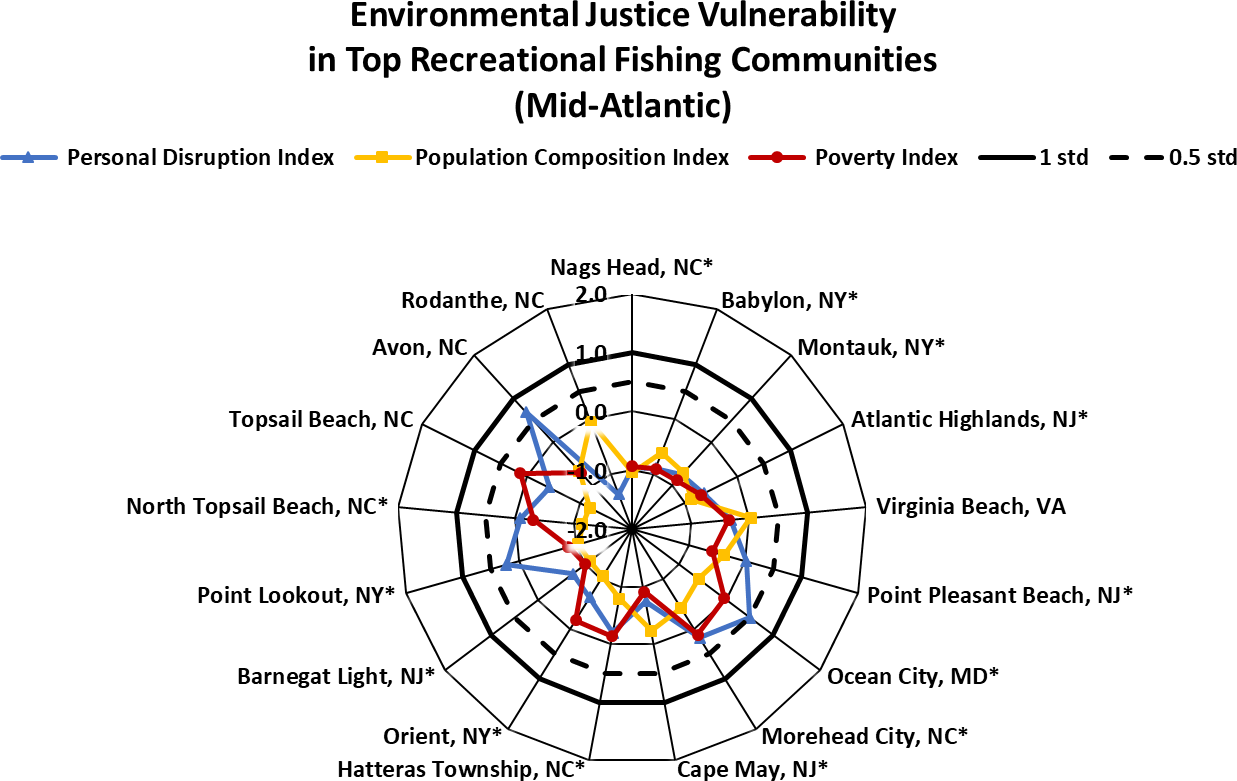
\includegraphics[width=0.75\linewidth]{SOE-MAFMC-2024_files/figure-latex/recreational-EJ-1} 

}

\caption{Environmental justice indicators (Poverty Index, population composition index, and personal disruption index) for top recreational fishing communities in Mid-Atlantic. Some communities are missing data for some indices. *Community scored high (1.00 and above) for both recreational engagement and reliance indicators.}\label{fig:recreational-EJ}
\end{figure}

\hypertarget{implications-4}{%
\subsubsection{Implications}\label{implications-4}}

A range of environmental justice concerns are found throughout Mid-Atlantic fishing communities. However, index scores for these concerns are higher overall in the top commercial communities relative to the top recreational communities.

These indicators provide a snapshot of the presence of environmental justice issues in the most highly engaged and most highly reliant commercial and recreational fishing communities in the Mid-Atlantic. These communities may be especially vulnerable to changes in fishing patterns due to regulations and/or climate change. Some changes occurred among the top fishing communities due to shifts in fishing activities, both commercial and recreational. Many of these communities, especially top commercial fishing communities, demonstrated medium to high environmental justice vulnerability, indicating that they may be at a disadvantage when responding to change.

\hypertarget{protected-species}{%
\subsection{Protected Species}\label{protected-species}}

Fishery management objectives for protected species generally focus on reducing threats and on habitat conservation/restoration. Protected species include marine mammals protected under the Marine Mammal Protection Act, endangered and threatened species protected under the Endangered Species Act, and migratory birds protected under the Migratory Bird Treaty Act. In the Northeast U.S., endangered/threatened species include Atlantic salmon, Atlantic and shortnose sturgeon, all sea turtle species, and five baleen whales. Protected species objectives include managing bycatch to remain below potential biological removal (PBR) thresholds, recovering endangered populations, and monitoring unusual mortality events (UMEs). Here we report on performance relative to these objectives with available indicator data, as well as indicating the potential for future interactions driven by observed and predicted ecosystem changes in the Northeast U.S.

\hypertarget{indicators-bycatch-population-adult-and-juvenile-numbers-mortalities}{%
\subsubsection{Indicators: bycatch, population (adult and juvenile) numbers, mortalities}\label{indicators-bycatch-population-adult-and-juvenile-numbers-mortalities}}

Average indices for both \href{https://noaa-edab.github.io/catalog/harborporpoise.html}{harbor porpoise} (Fig. \ref{fig:harborporpoise}) and \href{https://noaa-edab.github.io/catalog/grayseal.html}{gray seal} bycatch (Fig. \ref{fig:grayseal}) are below current PBR thresholds, meeting management objectives.

\begin{figure}

{\centering \includegraphics{SOE-MAFMC-2024_files/figure-latex/harborporpoise-1} 

}

\caption{Harbor porpoise average bycatch estimate for Mid-Atlantic and New England gillnet fisheries (blue) and the potential biological removal (red).}\label{fig:harborporpoise}
\end{figure}

The annual estimate for gray seal bycatch has declined since 2019, in part driven by declining gillnet landings. In addition, estimates since 2019 have greater uncertainty stemming from low observer coverage since 2019. The rolling mean confidence interval remains just below the PBR threshold.

\begin{figure}

{\centering \includegraphics{SOE-MAFMC-2024_files/figure-latex/grayseal-1} 

}

\caption{Gray Seal average bycatch estimate for gillnet fisheries (blue) and and the potential biological removal (red).}\label{fig:grayseal}
\end{figure}

The \href{https://noaa-edab.github.io/catalog/narw.html}{North Atlantic right whale population} was on a recovery trajectory until 2010, but has since declined (Fig. \ref{fig:narw-abundance}). The sharp decline observed from 2015-2020 appears to have slowed, although the right whale population continues to experience annual mortalities above recovery thresholds. Reduced survival rates of adult females lead to diverging abundance trends between sexes. It is estimated that there are fewer than 70 adult females remaining in the population.\\

\begin{figure}

{\centering \includegraphics{SOE-MAFMC-2024_files/figure-latex/narw-abundance-1} 

}

\caption{Estimated North Atlanic right whale abundance on the Northeast Shelf.}\label{fig:narw-abundance}
\end{figure}

North Atlantic right whale \href{https://noaa-edab.github.io/catalog/narw.html}{calf counts} have generally declined after 2009 to the point of having zero new calves observed in 2018 (Fig. \ref{fig:NARW-calf-abundance}). However, since 2019, we have seen more calf births each year with 15 births in 2022.

\begin{figure}

{\centering \includegraphics{SOE-MAFMC-2024_files/figure-latex/NARW-calf-abundance-1} 

}

\caption{Number of North Atlantic right whale calf births, 1990 - 2022.}\label{fig:NARW-calf-abundance}
\end{figure}

This year, the Unusual Mortality Event (UME) for North Atlantic right whales continued. From 2017 through 16 February 2024, the total UME right whale mortalities includes 38 dead stranded whales, 17 in the US and 21 in Canada. When alive but seriously injured whales (34) and sublethal injuries or ill whales (51) are taken into account, 123 individual whales are included in the UME. Recent research suggests that many mortalities go unobserved and the true number of mortalities are about three times the count of the observed mortalities. The primary cause of death is ``human interaction'' from entanglements or vessel strikes.

A UME continued from previous years for humpback whales (2016-present) and Atlantic minke whales (2018-present); suspected causes include human interactions. A UME for Northeast pinnipeds that began in 2018 for infectious disease is pending closure as of February 2024.

\hypertarget{implications-5}{%
\subsubsection{Implications}\label{implications-5}}

Bycatch management measures have been implemented to maintain bycatch below PBR thresholds. The downward trend in harbor porpoise bycatch could also be due to a decrease in harbor porpoise abundance in U.S. waters, reducing their overlap with fisheries, and a decrease in gillnet effort. The increasing trend in gray seal bycatch may be related to an increase in the gray seal population (\href{https://noaa-edab.github.io/catalog/seal_pups.html}{U.S. pup counts}), supported by the dramatic rise over the last three decades in observed numbers of gray seal pups born at U.S. breeding sites plus an increase in adult seals at the breeding sites, some of which are supplemented by Canadian adults.

Strong evidence exists to suggest that interactions between right whales and both the fixed gear fisheries in the U.S. and Canada and vessel strikes in the U.S. are contributing substantially to the decline of the species. Further, right whale distribution has changed since 2010. \href{https://noaa-edab.github.io/catalog/narw.html}{New research} suggests that recent climate driven changes in ocean circulation have resulted in right whale distribution changes driven by increased warm water influx through the Northeast Channel, which has reduced the primary right whale prey (the copepod Calanus finmarchicus) in the central and eastern portions of the Gulf of Maine. Additional potential stressors include offshore wind development, which overlaps with important habitat areas used year-round by right whales, including mother and calf migration corridors and foraging habitat. This area is also the only known right whale winter foraging habitat. Additional information can be found in the \protect\hyperlink{other-ocean-uses-offshore-wind}{offshore wind risks section}.

The UMEs are under investigation and are likely the result of multiple drivers. For all large whale UMEs, human interaction appears to have contributed to increased mortalities, although investigations are not complete.

A climate vulnerability assessment is published for Atlantic and Gulf of Mexico marine mammal populations.

\hypertarget{risks-to-meeting-fishery-management-objectives}{%
\section{Risks to Meeting Fishery Management Objectives}\label{risks-to-meeting-fishery-management-objectives}}

\hypertarget{climate-and-ecosystem-change}{%
\subsection{Climate and Ecosystem Change}\label{climate-and-ecosystem-change}}

Regulations and measures designed to meet fishery management objectives are often based on historical information about stocks, their distribution in space and time, and their overall productivity. Large scale climate related changes in the ecosystem can lead to changes in important habitats and ecological interactions, altering distributions and productivity. With large enough ecosystem changes, management measures may be less effective, and management objectives may not be met.

This year, we have restructured this section to focus on three categories of management decisions and the risk posed to them by climate and ecosystem change: spatial management, seasonal management, and quota setting or rebuilding depleted stocks. In each section, we describe potential risks to a management category, highlight indicators of observed changes that contribute to those risks, review possible biological and environmental drivers and the ways they may explain the observed indicators, and raise potential future implications if these trends persist or change.

\hypertarget{risks-to-spatial-management}{%
\subsubsection{Risks to Spatial Management}\label{risks-to-spatial-management}}

Shifting species distributions (changes in spatial extent or center of gravity) alter both species interactions and fishery interactions. In particular, shifting species distributions can affect expected management outcomes from spatial allocations and bycatch measures based on historical fish and protected species distributions. Species availability to surveys can also change as distributions shift within survey footprints.

\hypertarget{indicators-fish-and-protected-species-distribution-shifts}{%
\paragraph{Indicators: Fish and protected species distribution shifts}\label{indicators-fish-and-protected-species-distribution-shifts}}

As noted in the \protect\hyperlink{implications}{Landings Implications section above}, the center of \href{https://noaa-edab.github.io/catalog/species_dist.html}{distribution} for a suite of 48 commercially or ecologically important fish species along the entire Northeast Shelf continues to show movement towards the northeast and generally into deeper water (Fig. \ref{fig:species-dist}).

\begin{figure}

{\centering \includegraphics{SOE-MAFMC-2024_files/figure-latex/species-dist-1} 

}

\caption{Aggregate species distribution metrics for species in the Northeast Large Marine Ecosystem: along shelf distance with increasing trend (orange), and depth with decreasing trend indicating deeper water (purple).}\label{fig:species-dist}
\end{figure}

\href{https://noaa-edab.github.io/catalog/habitat_diversity.html}{Habitat model-based species richness} suggests shifts of both cooler and warmer water species to the northeast. Similar patterns have been found for \href{https://noaa-edab.github.io/catalog/HMS_species_distribution.html}{marine mammals}, with multiple species shifting northeast between 2010 and 2017 in most seasons (Fig. \ref{fig:protectedspp-dist-shifts}).

\begin{figure}

{\centering \includegraphics{SOE-MAFMC-2024_files/figure-latex/protectedspp-dist-shifts-1} 

}

\caption{Direction and magnitude of core habitat shifts, represented by the length of the line of the seasonal weighted centroid for species with more than 70 km difference between 2010 and 2017 (tip of arrow).}\label{fig:protectedspp-dist-shifts}
\end{figure}

\hypertarget{drivers}{%
\paragraph{Drivers:}\label{drivers}}

Mobile populations shift distributions to maintain suitable temperature and prey fields, possibly expanding ranges if new suitable habitat exists. Changes in managed species distribution is related, in part, to the \href{https://noaa-edab.github.io/catalog/forage_index.html}{distribution of forage biomass}. Since 1982, the fall center of gravity of forage fish (20 species combined) has moved to the north and east (Fig. \ref{fig:forageshifts}). Spring forage fish center of gravity has been more variable over time.

\begin{figure}

{\centering \includegraphics{SOE-MAFMC-2024_files/figure-latex/forageshifts-1} 

}

\caption{Eastward (left) and northward (right) shifts in the center of gravity for 20 forage fish species on the Northeast U.S. Shelf, with increasing trend (orange) for fall eastward and northward center of gravity.}\label{fig:forageshifts}
\end{figure}

Ocean temperatures influence the distribution, seasonal timing, and productivity of managed species (see sections below). The Northeast US shelf, including the Mid-Atlantic, has experienced a continued warming trend for both the \href{https://noaa-edab.github.io/catalog/long_term_sst.html}{long term} (Fig. \ref{fig:long-term-sst}) and \href{https://noaa-edab.github.io/catalog/seasonal_oisst_anom.html}{recent surface} and \href{https://noaa-edab.github.io/catalog/bottom_temp_comp.html}{bottom} in all seasons.

\begin{figure}

{\centering \includegraphics{SOE-MAFMC-2024_files/figure-latex/long-term-sst-1} 

}

\caption{Northeast US annual sea surface temperature (SST, black), with increasing trend (orange).}\label{fig:long-term-sst}
\end{figure}

Species suitable habitat can expand or contract when changes in temperature and major oceanographic conditions alter distinct water mass habitats.The variability of the Gulf Stream is a major driver of the predominant oceanographic conditions of the Northeast U.S. continental shelf. As the \href{https://noaa-edab.github.io/catalog/gsi.html}{Gulf Stream} has become less stable and shifted northward in the last decade (Fig. \ref{fig:GSI}), warmer ocean temperatures have been observed on the northeast shelf and a higher proportion of \href{https://noaa-edab.github.io/catalog/slopewater.html}{Warm Slope Water} has been present in the Northeast Channel.

\begin{figure}

{\centering \includegraphics{SOE-MAFMC-2024_files/figure-latex/GSI-1} 

}

\caption{Index representing changes in the location of the Gulf Stream north wall (black). Positive values represent a more northerly Gulf Stream position, with increasing trend (orange).}\label{fig:GSI}
\end{figure}

Changes in ocean temperature and circulation alter habitat features such as the seasonal \href{https://noaa-edab.github.io/catalog/cold_pool.html}{cold pool}, a band of relatively cold near-bottom water from spring to fall over the northern MAB. The cold pool represents essential fish spawning and nursery habitat, and affects fish distribution and behavior. The cold pool has been getting warmer and smaller over time (Fig. \ref{fig:cold-pool-size}). The spatial extent (or area) of the seasonal cold pool is decreasing over time, yet the interannual variability of cold pool area has increased.

\begin{figure}

{\centering \includegraphics{SOE-MAFMC-2024_files/figure-latex/cold-pool-size-1} 

}

\caption{Seasonal cold pool mean temperature (left) and spatial extent index (right), based on bias-corrected ROMS-NWA (open circles) and GLORYS (closed circles), with declining trends (purple).}\label{fig:cold-pool-size}
\end{figure}

\hypertarget{future-considerations}{%
\paragraph{Future Considerations}\label{future-considerations}}

Distribution shifts caused by changes in thermal habitat are likely to continue as long as long-term temperature trends persist. Near-term oceanographic forecasts are currently in development and may inform how future warming impacts species distributions.

Distribution patterns associated with climate-driven changes in ocean circulation are also unlikely to be reversed to historical ranges in the short term. Increased oceanographic variability needs to be captured by regional ocean models and linked to species distribution processes to better understand potential future distributions. Species with high mobility or short lifespans react differently from immobile or long lived species.

Adapting management to changing stock distributions and dynamic ocean processes will require continued monitoring of populations in space and evaluating management measures against a range of possible future spatial distributions. Processes like the \href{https://www.mafmc.org/climate-change-scenario-planning}{East Coast Climate Scenario Planning} can help coordinate management.

\hypertarget{risks-to-seasonal-management}{%
\subsubsection{Risks to Seasonal Management}\label{risks-to-seasonal-management}}

The effectiveness of seasonal management actions (fishing seasons or area opening/closing) depends on a proper alignment with the seasonal life cycle events (phenology) of fish stocks (e.g.~migration timing and spawning). Changes in the timing of these biological cycles can reduce the effectiveness of management measures if not accounted for. The timing of seasonal patterns can also change the interactions between fisheries and non-target species thus influencing the amount of bycatch and the availability of species to surveys.

\hypertarget{indicators-timing-shifts}{%
\paragraph{Indicators: Timing shifts}\label{indicators-timing-shifts}}

\href{https://noaa-edab.github.io/catalog/spawn_timing.html}{Spawning timing} is shifting earlier for multiple stocks, including haddock and yellowtail flounder. Spawning of both haddock stocks occurred earlier in the year, as indicated by more resting (post-spawning) stage fish in the 2010s as compared to earlier in the time series (Fig. \ref{fig:spawntiming}). The northern (CC/GOM) stock shows earlier active spawning in recent years with a decline in pre-spawning resting females.The recent increase in resting females in the southern (SNE) stock also indicates a shift to earlier spawning (i.e.~more post-spawn fish). Yellowtail flounder spawning is related to bottom temperature, week of year, and decade sampled for each of the three stocks.

\begin{figure}

{\centering \includegraphics{SOE-MAFMC-2024_files/figure-latex/spawntiming-1} 

}

\caption{Percent resting stage (non-spawning) mature female fish (black) with significant increases (orange) and decreases (purple) from two haddock and three yellowtail flounder stocks: CC = Cape Cod Gulf of Maine, GOM = Gulf of Maine, GB = Georges Bank, SNE = Southern New England. }\label{fig:spawntiming}
\end{figure}

\href{https://noaa-edab.github.io/catalog/timing_shifts.html}{Migration timing} of some tuna and large whale migrations has changed. For example, tuna were caught in recreational fisheries 50 days earlier in the year in 2019 compared to 2002. In Cape Cod Bay, peak spring habitat use by right and humpback whales has shifted 18-19 days later over time.

Understanding whether seasonal patterns are changing for stocks requires regular observations throughout the year. Despite the importance of understanding seasonal patterns, we have few indicators that directly assess timing shifts of species. We plan on incorporating more indicators of timing shifts and phenology in future reports.

\hypertarget{drivers-1}{%
\paragraph{Drivers:}\label{drivers-1}}

The drivers of timing shifts in managed stocks are generally coupled to shifts in environmental or biological conditions, since these can result in changes in habitat quality or food availability within the year. Changes in the timing of fall phytoplankton blooms and seasonal shifts in zooplankton communities are thought to be critical indicators of changes in seasonal food availability to stocks.

Along with the overall warming trends in the Mid Atlantic, ocean summer conditions have been lasting longer, as shown by the later \href{https://noaa-edab.github.io/catalog/trans_dates.html}{transition} from warm stratified summer conditions to well mixed cool fall conditions (Fig. \ref{fig:transition}). Changes in the broad seasonal cycles of their environment can lead to changes in species biological processes (migrations, spawning, etc.) that are triggered by seasonal events.

\begin{figure}

{\centering \includegraphics{SOE-MAFMC-2024_files/figure-latex/transition-1} 

}

\caption{Ocean summer length in the MAB: the annual total number of days between the spring thermal transition date and the fall thermal transition date (black), with an increasing trend (orange).}\label{fig:transition}
\end{figure}

The \href{https://noaa-edab.github.io/catalog/cold_pool.html}{cold pool} is a seasonal feature within the MAB that creates seasonally suitable habitat for many species. In 8 of the past 10 years, cold pool persistence has been well below average, so this habitat was available for a shorter portion of the year (Fig. \ref{fig:cold-pool-time}). A change in the timing of the cold pool may impact the recruitment of species that depend on it for juvenile habitat, such as yellowtail flounder.

\begin{figure}

{\centering \includegraphics{SOE-MAFMC-2024_files/figure-latex/cold-pool-time-1} 

}

\caption{Cold pool persistence index based on bias-corrected ROMS-NWA (open circles) and GLORYS (closed circles).}\label{fig:cold-pool-time}
\end{figure}

\hypertarget{future-considerations-1}{%
\paragraph{Future Considerations}\label{future-considerations-1}}

For stocks reliant on environmental processes to dictate the timing of their behavior (e.g.~phytoplankton bloom timing, thermal transition, or the duration of the cold pool), it is possible that some changes are episodic and have interannual variability, while other effects on timing can change on scales of years to decades. However, other species may rely on the general seasonal succession of their environment, which exhibits long-term trends unlikely to reverse in coming years. For those species, timing shifts in migration or spawning may continue. Management actions that rely on effective alignment of fisheries availability and biological processes should continue to evaluate whether prior assumptions on seasonal timings still hold, and new indicators should be developed to monitor timing shifts for stocks.

\hypertarget{risks-to-quota-settingrebuilding}{%
\subsubsection{Risks to Quota Setting/Rebuilding}\label{risks-to-quota-settingrebuilding}}

The efficacy of short-term stock projections and rebuilding plans rely on an accurate understanding of processes affecting stock growth, reproduction, and natural mortality. These biological processes are often driven by underlying environmental change. When observed environmental change occurs, there is a risk that established stock-level biological reference points may no longer reflect the current population.

\hypertarget{indicators-fish-productivity-and-condition-shifts}{%
\paragraph{Indicators: Fish productivity and condition shifts}\label{indicators-fish-productivity-and-condition-shifts}}

Indicators of \href{https://noaa-edab.github.io/catalog/productivity_anomaly.html}{fish productivity} are derived from observations (surveys) or models (stock assessments). Fish productivity has been declining in the Mid-Atlantic since the early 2000s, as described by the small-fish-per-large-fish anomaly indicator (derived from NEFSC bottom trawl survey) (Fig. \ref{fig:productivity-anomaly}). This decline in fish productivity is also shown by a similar analysis based on stock assessment model outputs (recruitment per spawning stock biomass anomaly).

\begin{figure}

{\centering \includegraphics{SOE-MAFMC-2024_files/figure-latex/productivity-anomaly-1} 

}

\caption{Fish productivity measures. Left: Small fish per large fish survey biomass anomaly in the Mid-Atlantic Bight. Right: assessment recruitment per spawning stock biomass anomaly for stocks mainly in the Mid-Atlantic. The summed anomaly across species is shown by the black line, drawn across all years with the same number of stocks analyzed.}\label{fig:productivity-anomaly}
\end{figure}

The health of individual fish (i.e.~fish condition) can contribute to population productivity through improved growth, reproduction and survival. \href{https://noaa-edab.github.io/catalog/condition.html}{Fish condition} in the MAB was generally good prior to 2000, poor from 2001-2010 (concurrent with declines in productivity, Fig. \ref{fig:productivity-anomaly}), and a mix of good and poor since 2011. In 2023, condition was mixed, with general improvement since a relatively low condition year in 2021 (Fig. \ref{fig:mab-cf}). Preliminary analyses show that changes in temperature, zooplankton, fishing pressure, and population size influence the condition of different fish species.

\begin{figure}

{\centering \includegraphics{SOE-MAFMC-2024_files/figure-latex/mab-cf-1} 

}

\caption{Condition factor for fish species in the MAB based on fall NEFSC bottom trawl survey data. MAB data are missing for 2017 due to survey delays, and no survey was conducted in 2020.}\label{fig:mab-cf}
\end{figure}

\hypertarget{drivers-2}{%
\paragraph{Drivers:}\label{drivers-2}}

Fish productivity and condition are affected by increasing metabolic demands from increasing temperature, combined with changes in the availability and quality of prey. Long-term environmental trends and episodic extreme temperatures, ocean acidification, and low oxygen events represent multiple stressors that can affect growth rates, reproductive success, recruitment, and cause mortality.

\hypertarget{biological-drivers-forage-quality-and-abundance}{%
\subparagraph{Biological Drivers: Forage quality and abundance}\label{biological-drivers-forage-quality-and-abundance}}

The amount of forage fish available in the ecosystem combined with the energy content of the forage species determines the amount of energy potentially available to predators in the ecosystem. Changes in the forage base can drive managed and protected species production.

The \href{https://noaa-edab.github.io/catalog/energy_density.html}{energy content} of juvenile and adult forage fish as prey is related to forage fish growth and reproductive cycles, as well as environmental conditions. The energy content of Atlantic herring from the NEFSC trawl surveys has increased recently (Fig. \ref{fig:energy-density}) but is still well below that observed in the 1980s and 1990s. Silver hake, longfin squid (Loligo in figure) and shortfin squid (Illex in figure) remain lower than previous estimates.

\begin{figure}

{\centering \includegraphics{SOE-MAFMC-2024_files/figure-latex/energy-density-1} 

}

\caption{Forage fish energy density mean and standard deviation by season and year, compared with 1980s (solid line) and 1990s (dashed line) values.}\label{fig:energy-density}
\end{figure}

Changes in the overall abundance of forage fish can influence managed species productivity as it relates to changes in food availability. A spatially-explicit \href{https://noaa-edab.github.io/catalog/forage_index.html}{forage index} for the Mid-Atlantic shows a long term declining trend in fall, with higher forage biomass in fall than spring (Fig. \ref{fig:foragebio}). Forage biomass was highest during fall in the early-1980s.\\

\begin{figure}

{\centering \includegraphics{SOE-MAFMC-2024_files/figure-latex/foragebio-1} 

}

\caption{Forage fish index in the MAB for spring (blue) and fall (red) surveys, with a decline (purple) in fall. Index values are relative to the maximum observation within a region across surveys.}\label{fig:foragebio}
\end{figure}

\hypertarget{biological-drivers-lower-trophic-levels}{%
\subparagraph{Biological Drivers: Lower trophic levels}\label{biological-drivers-lower-trophic-levels}}

\href{https://noaa-edab.github.io/catalog/chl_pp.html}{Phytoplankton} are the foundation of the food web and are the primary food source for zooplankton and filter feeders such as shellfish. Numerous environmental and oceanographic factors affect the abundance, \href{https://noaa-edab.github.io/catalog/phyto_size.html}{size composition}, spatial distribution, and productivity of phytoplankton. While changes in fish productivity (including forage) could result from changing primary productivity, total primary production in the Mid Atlantic has no clear trend (Fig. \ref{fig:totpp}).

\href{https://noaa-edab.github.io/catalog/zoo_abundance_anom.html}{Zooplankton} communities in the Mid-Atlantic have increasing trends for smaller bodied copepods and gelatinous species (Cnidaria; Fig. \ref{fig:zoopanom}). Smaller bodied copepods and gelatinous species are less energy-rich than Eupausiids (krill) or the larger-bodied copepod \emph{Calanus finmarchicus}. A changing mix of zooplankton prey can impact forage fish energy content and abundance, as well as the prey field of filter feeding whales.

\begin{figure}

{\centering \includegraphics{SOE-MAFMC-2024_files/figure-latex/zoopanom-1} 

}

\caption{Changes in zooplankton abundance in the MAB for large (top left) and small (top right) copepods, Cnidarians (bottom left), and Euphausiids (bottom right), with significant increases (orange) in small copeods and Cnidarians.}\label{fig:zoopanom}
\end{figure}

\hypertarget{environmental-drivers}{%
\subparagraph{Environmental Drivers}\label{environmental-drivers}}

Fish production can also be directly related to the prevailing environmental conditions by altering metabolic processes (growth) and reproduction. Many species possess thermal tolerances and can experience stressful or lethal conditions if temperatures exceed certain levels. Extreme temperatures at both the \href{https://noaa-edab.github.io/catalog/seasonal_oisst_anom.html}{surface} and \href{https://noaa-edab.github.io/catalog/bottom_temp_comp.html}{bottom} can exceed \href{https://noaa-edab.github.io/catalog/thermal_habitat_persistence.html}{thermal tolerance} limits for some fish. For example, 2015 had the \href{https://noaa-edab.github.io/catalog/bottom_temp_comp.html}{warmest summer and fall bottom temperatures} in the Mid-Atlantic. A large proportion of the region had bottom temperatures above the 15℃ thermal tolerance for most groundfish, with some days exceeding the 24℃ potential mortality limit (Fig. \ref{fig:therm-hab-persist-2015}). Many Mid-Atlantic species have different thermal tolerance limits from groundfish, and we will work to include those next year.

\begin{figure}

{\centering 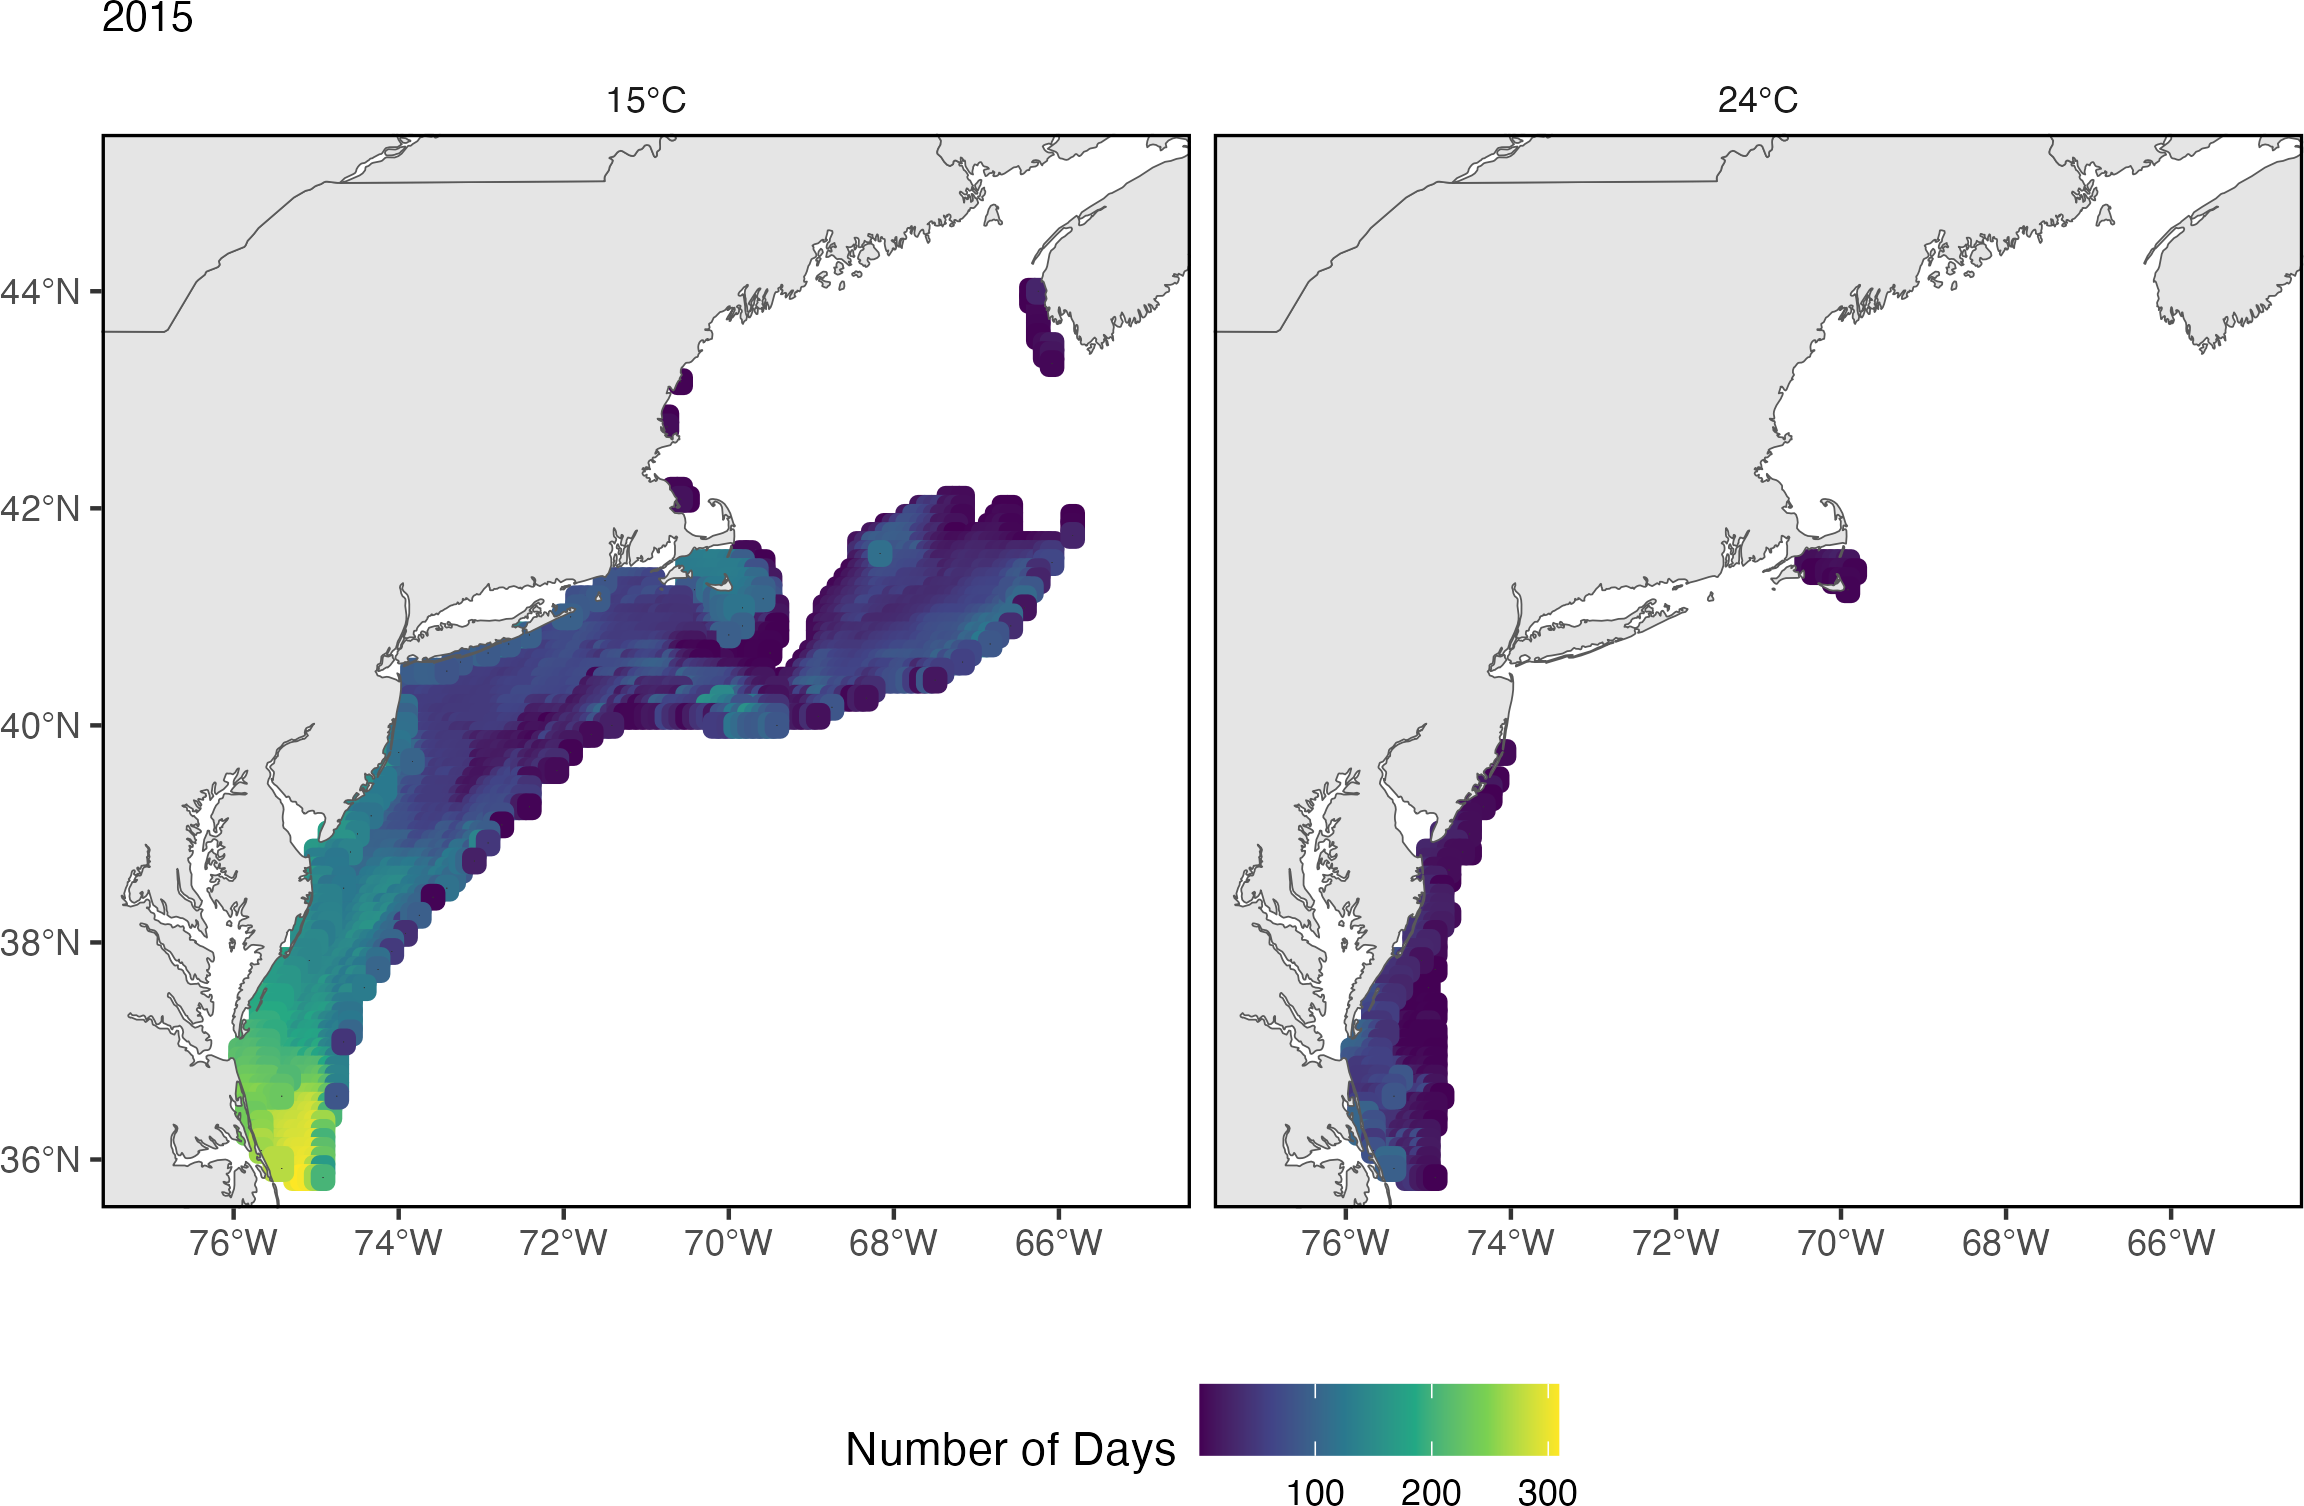
\includegraphics[width=0.9\linewidth]{images/thermal_habitat_2015_cropped} 

}

\caption{The number of days in 2015 where bottom temperature exceeds 15℃ (left) and 24℃ (right) based on the GLORYS 1/12 degree grid.}\label{fig:therm-hab-persist-2015}
\end{figure}

\href{https://noaa-edab.github.io/catalog/ocean_acidification.html}{Ocean acidification} (OA) risks vary among species and include reduced survival, growth, reproduction, and productivity, where high OA risk indicates potential negative effects to species. High OA risk conditions were observed for Atlantic sea scallop and longfin squid in Long Island Sound and the nearshore and mid shelf regions of the New Jersey shelf during summer of 2016, 2018, 2019, and 2023 (Fig. \ref{fig:mab-oa}).

\begin{figure}

{\centering 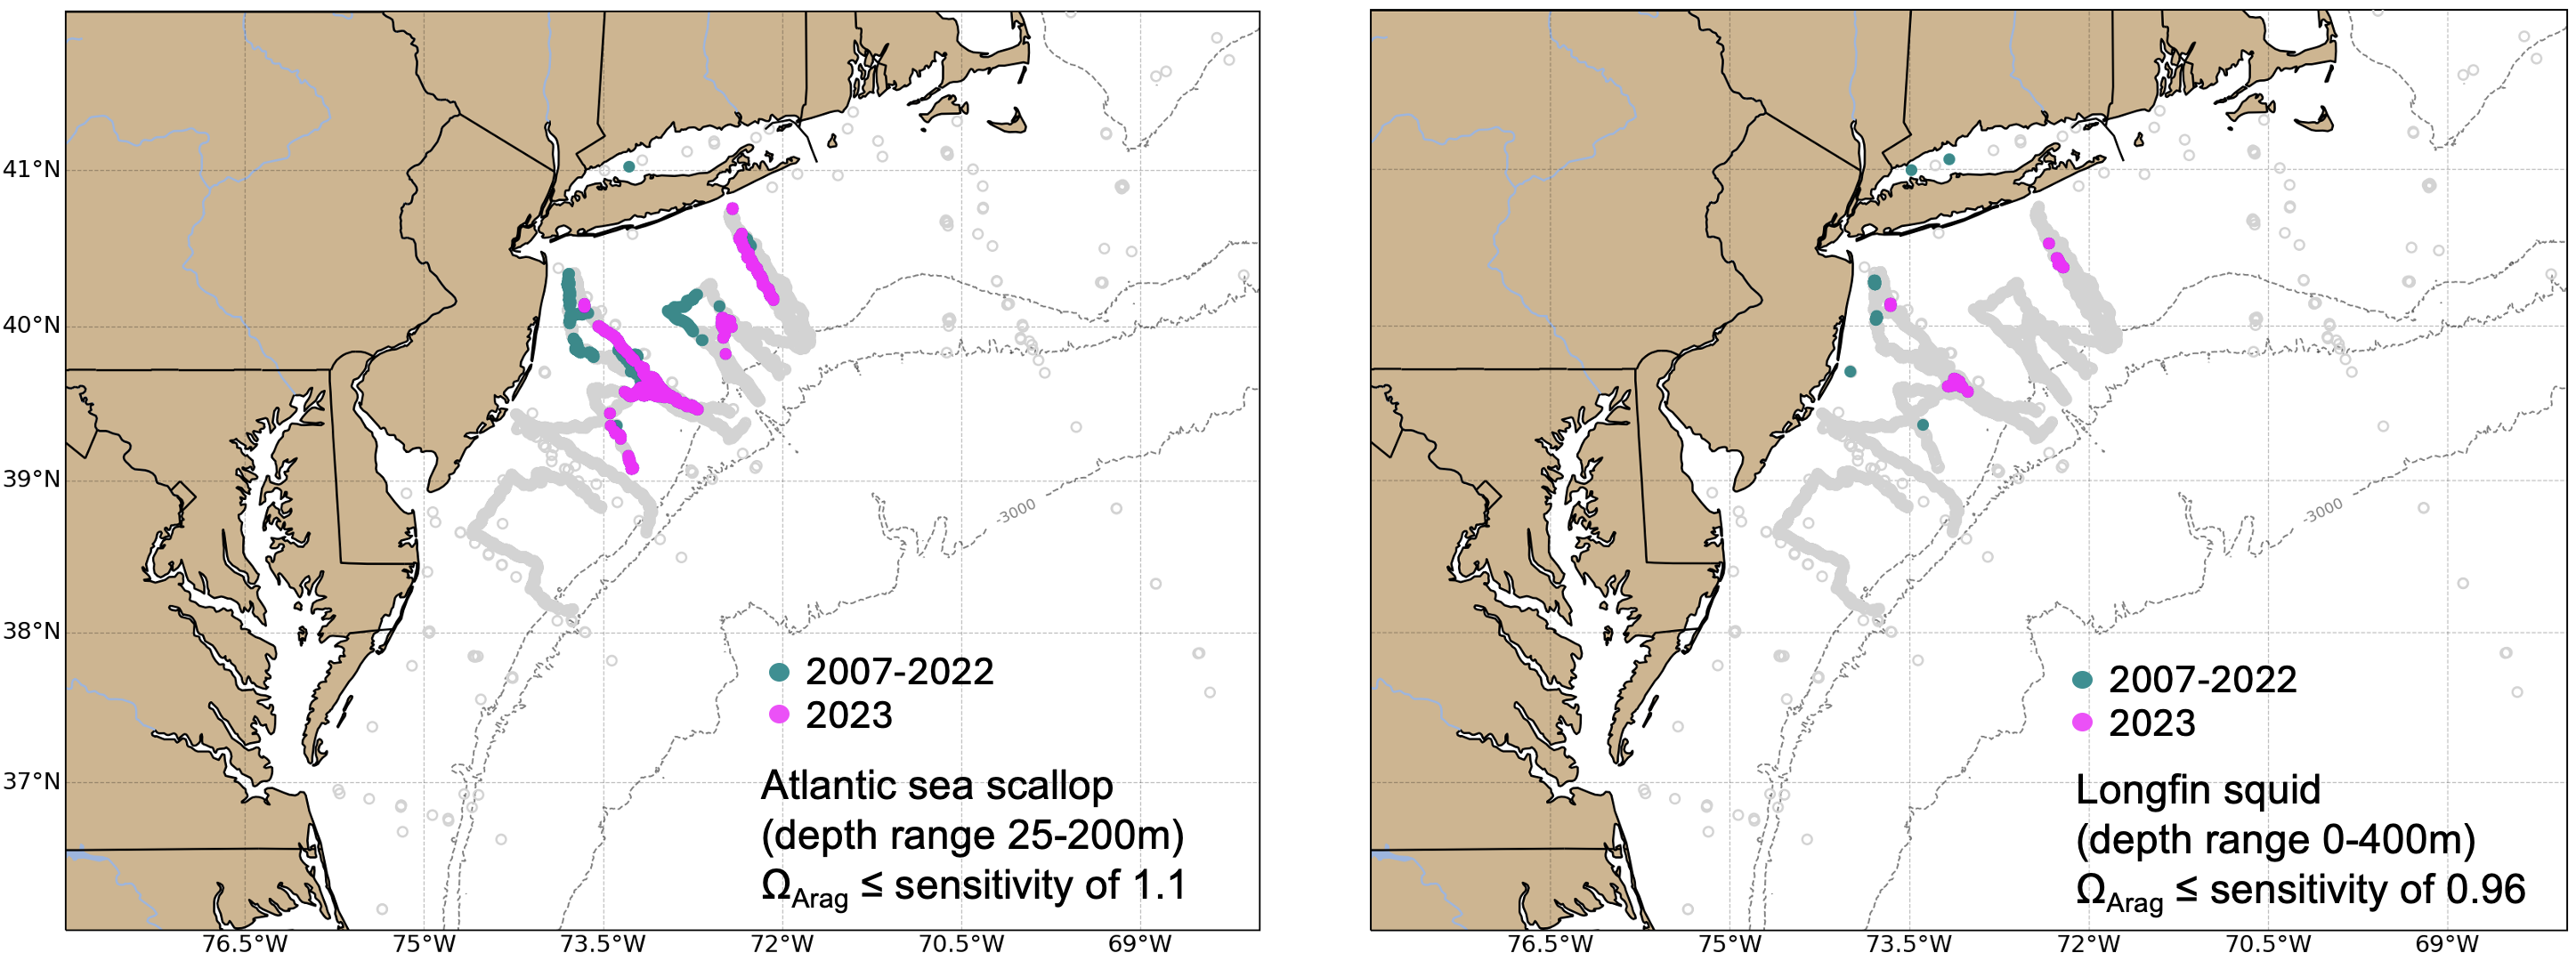
\includegraphics[width=1\linewidth]{SOE-MAFMC-2024_files/figure-latex/mab-oa-1} 

}

\caption{Locations where bottom aragonite saturation state ($\Omega_{Arag}$; summer only: June-August) were at or below the laboratory-derived sensitivity level for Atlantic sea scallop (left panel) and longfin squid (right panel) for the time periods 2007-2022 (dark cyan) and 2023 only (magenta). Gray circles indicate locations where bottom $\Omega_{Arag}$ values were above the species specific sensitivity values..}\label{fig:mab-oa}
\end{figure}

Biological and oceanographic processes can affect the amount of oxygen present in the water column. During low oxygen (hypoxic) events, species growth is negatively affected, and very low oxygen can result in mortality. The duration and extent of hypoxic events is being monitored, but long-term shelf-wide observations are not yet available. However, \href{https://noaa-edab.github.io/catalog/ocean_acidification.html}{hypoxic events} were detected off the coast of New Jersey in 2023 and were potentially responsible for fish, lobster, and crab \href{https://sebsnjaesnews.rutgers.edu/2023/12/rutgers-scientists-observe-unusual-ocean-conditions-possibly-linked-to-mortality-in-marine-life-off-new-jersey/}{mortalities}.

\hypertarget{drivers-predation}{%
\paragraph{Drivers: Predation}\label{drivers-predation}}

The abundance and distribution of predators can affect both the productivity and mortality rates on managed stocks. Predators can consume managed species or compete for the same resources, resulting in increased natural mortality or decreased productivity. The northeast shift in \href{https://noaa-edab.github.io/catalog/HMS_species_distribution.html}{whales and dolphins} (Fig. \ref{fig:protectedspp-dist-shifts}) indicates a change in the overlap between predators and prey. Since we also observe distribution shifts in managed species as well as forage species, the effect of changing predator distributions alone is difficult to quantify.

Indicators for shark populations, combined with information on gray seals (see \protect\hyperlink{protected-species}{Protected Species Implications section, above}), suggests predator populations range from stable (\href{https://noaa-edab.github.io/catalog/hms_cpue.html}{sharks}) to increasing (\href{https://noaa-edab.github.io/catalog/seal_pups.html}{gray seals}) in the MAB. \href{https://noaa-edab.github.io/catalog/hms_stock_status.html}{Stock status} is mixed for Atlantic Highly Migratory Species (HMS) stocks (including sharks, swordfish, billfish, and tunas) occurring throughout the Northeast U.S. shelf. While there are several HMS species considered to be overfished or that have unknown stock status, the population status for some managed Atlantic sharks and tunas is at or above the biomass target, suggesting the potential for robust predator populations among these managed species. Stable predator populations suggest stable predation pressure on managed species, but increasing predator populations may reflect increasing predation pressure.

\hypertarget{future-considerations-2}{%
\subsubsection{Future Considerations}\label{future-considerations-2}}

The processes that control fish productivity and mortality are dynamic, complex, and are the result of the interactions between multiple system drivers. There is a real risk that short-term predictions in assessments and rebuilding plans that assume unchanging underlying conditions will not be as effective, given the observed change documented in the prior sections in both ecological and environmental processes. Assumptions for species' growth, reproduction, and natural mortality should continue to be evaluated for individual species. With observations of system-wide productivity shifts of multiple managed stocks, more research is needed to determine whether regime shifts or ecosystem reorganization are occurring, and how this should be incorporated into management.

\hypertarget{other-ocean-uses-offshore-wind}{%
\subsection{Other Ocean Uses: Offshore Wind}\label{other-ocean-uses-offshore-wind}}

\hypertarget{indicators-development-timeline-revenue-in-lease-areas-coastal-community-vulnerability}{%
\subsubsection{Indicators: development timeline, revenue in lease areas, coastal community vulnerability}\label{indicators-development-timeline-revenue-in-lease-areas-coastal-community-vulnerability}}

As of January 2024, 30 offshore \href{https://noaa-edab.github.io/catalog/wind_dev_speed.html}{wind development} projects are proposed for construction over the next decade in the Northeast (timelines and project data for 2024 are based on the Ocean Wind 1 Offshore Wind Farm Final Environmental Impact Statement. Volume II: Appendix F). Offshore wind areas are anticipated to cover more than 2.3 million acres by 2030 in the Greater Atlantic region (Fig. \ref{fig:wind-proposed-dev}). All states will be able to reach their 2030 offshore wind goals with existing lease areas.\\

\begin{figure}

{\centering \includegraphics{SOE-MAFMC-2024_files/figure-latex/wind-proposed-dev-1} 

}

\caption{Total area proposed for wind develpment on the northeast shelf through 2030.}\label{fig:wind-proposed-dev}
\end{figure}

Just over 3,300 foundations and more than 12,000 miles of inter-array and offshore export cables are proposed to date (Fig. \ref{fig:wind-dev-cumul}). Based on current timelines, the areas affected would be spread out such that it is unlikely that any one particular area would experience full development at one time. Construction of two projects in Southern New England (South Fork Wind and Vineyard Wind 1) during 2023 affected fisheries managed by the Mid-Atlantic Fishery Management Council, while construction activities began for Revolution Wind in early 2024. It is likely that construction will begin on other projects in Southern New England and possibly the New York Bight during 2024 that will further affect regional fisheries.

\begin{figure}

{\centering 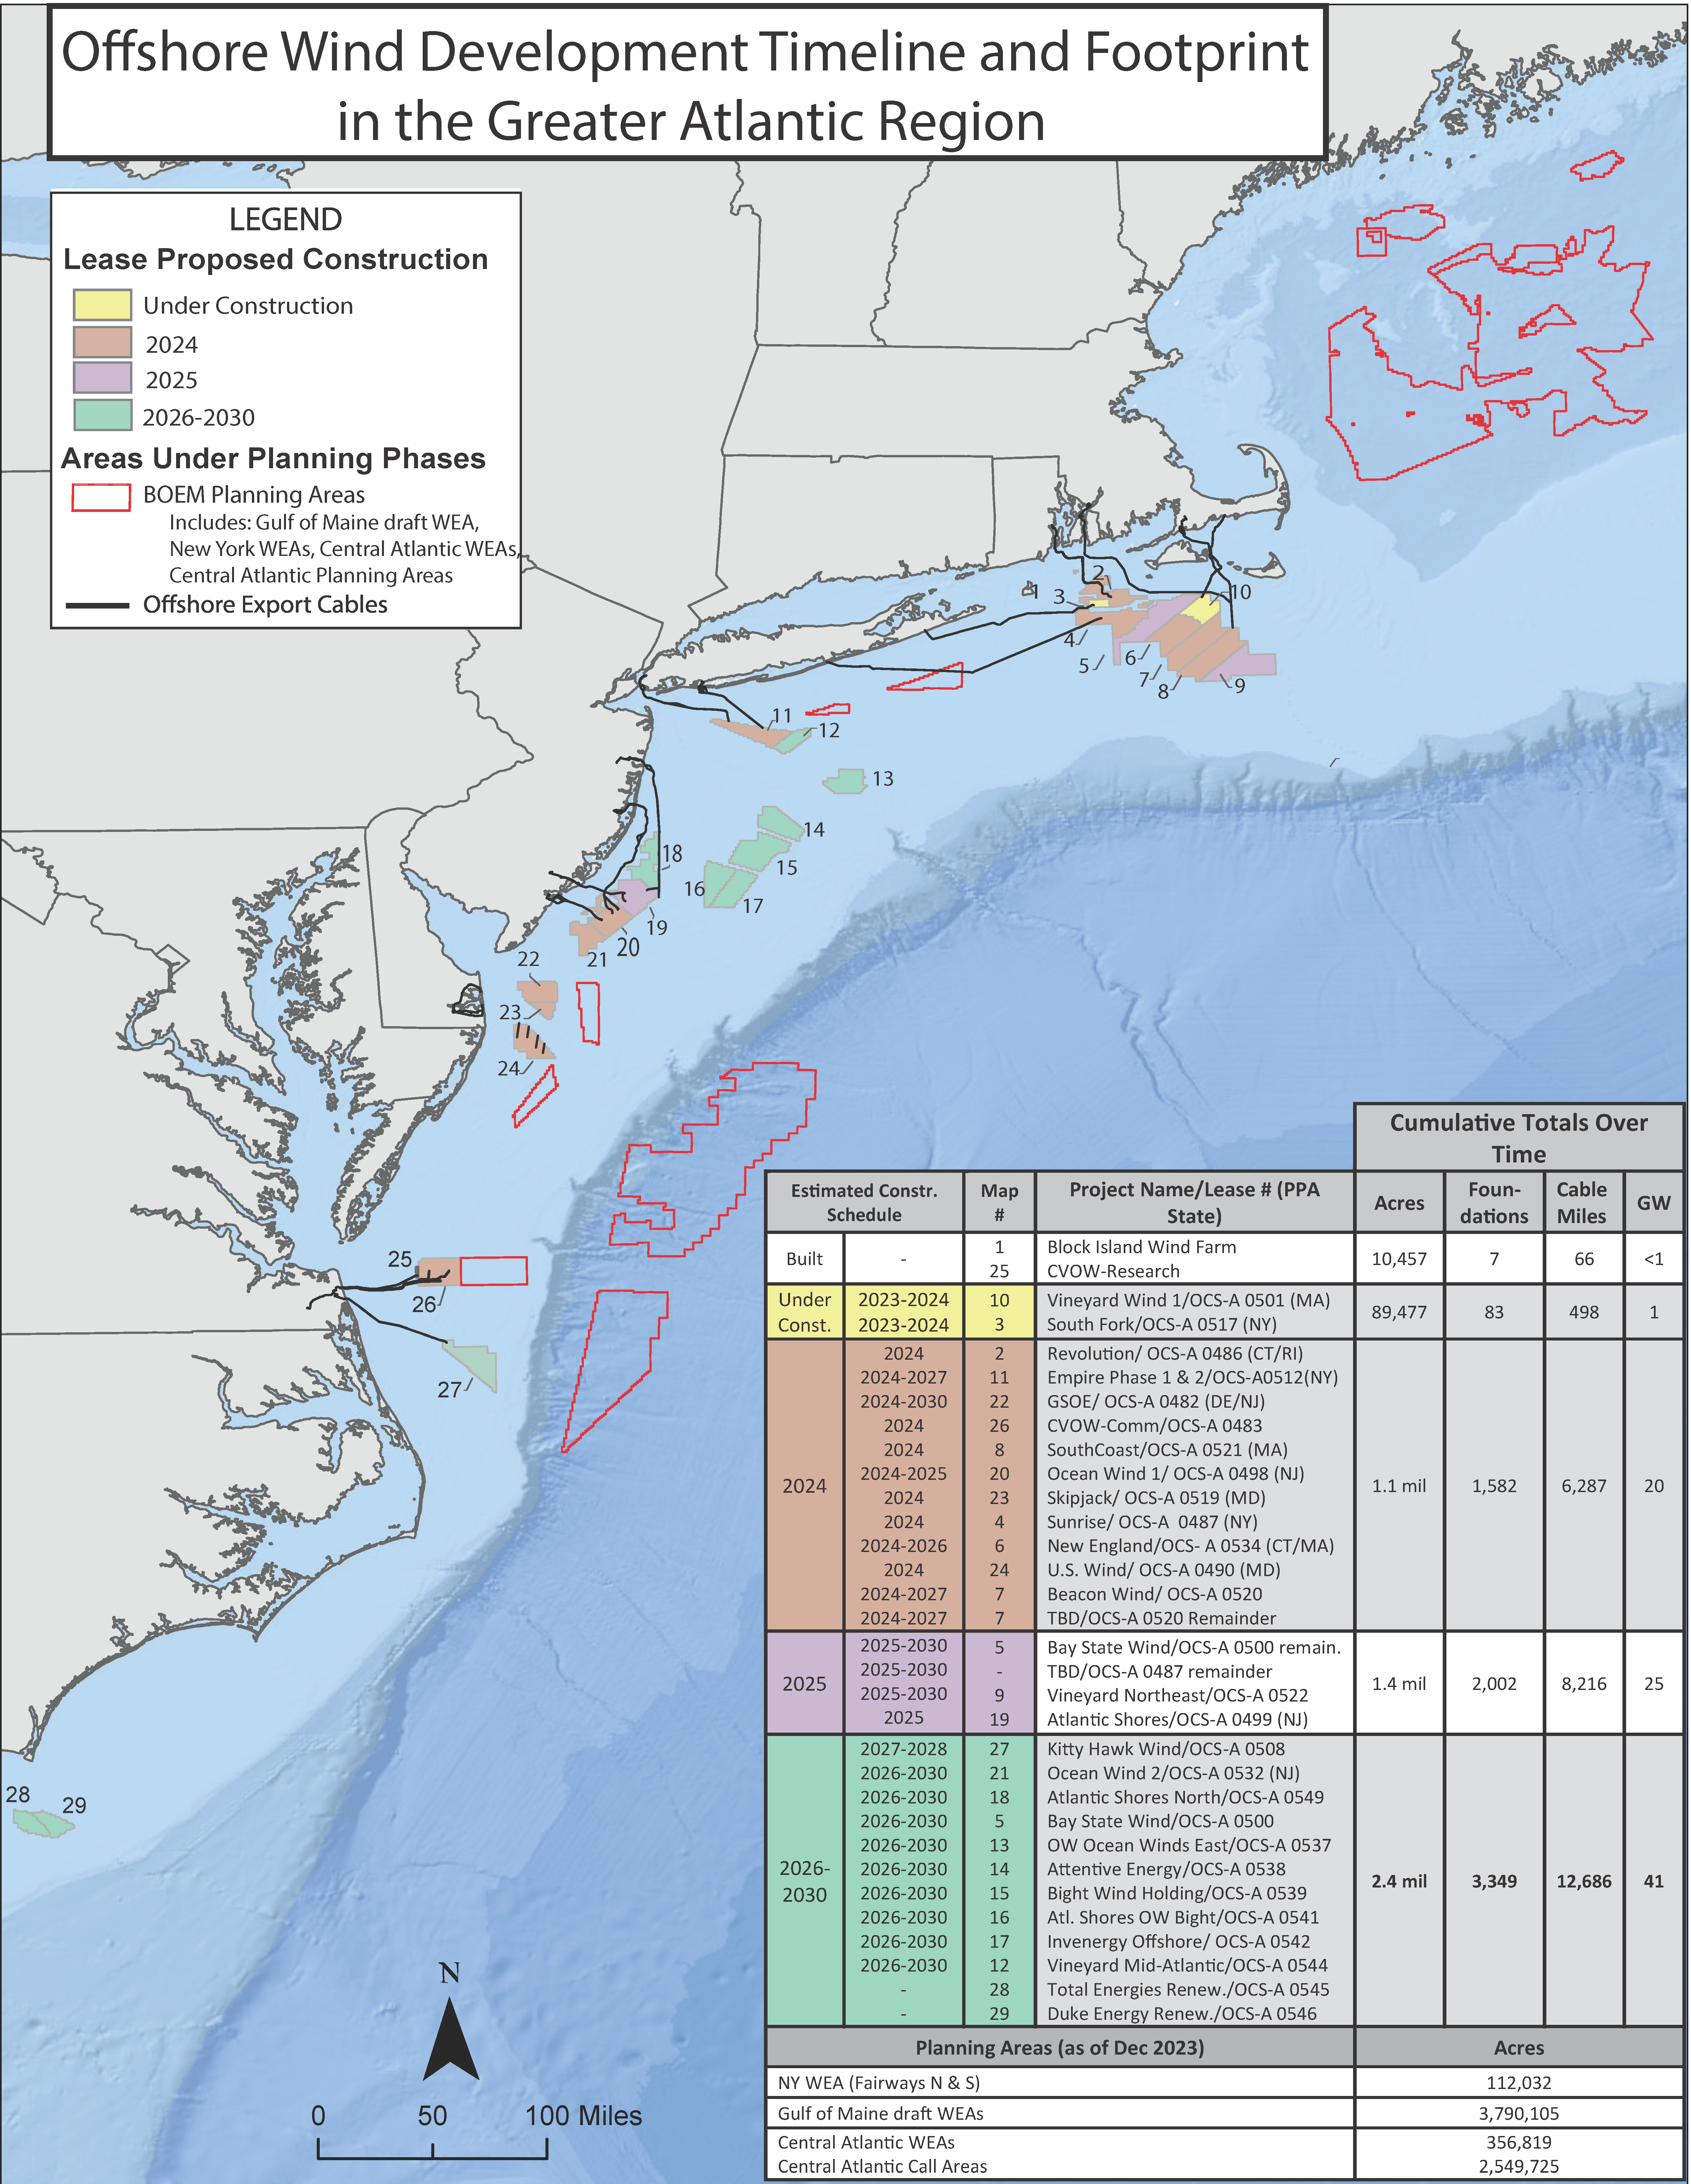
\includegraphics[width=0.9\linewidth]{SOE-MAFMC-2024_files/figure-latex/wind-dev-cumul-1} 

}

\caption{All Northeast Project areas by year construction ends (each project has 2 year construction period).}\label{fig:wind-dev-cumul}
\end{figure}

Based on federal vessel logbook data, \href{https://noaa-edab.github.io/catalog/wind_revenue.html}{commercial fishery revenue} from trips in the current offshore wind lease areas, including the newly designated lease areas in the Central Atlantic, have varied annually from 2008-2022, with less than \$1 million in maximum annual revenue overlapping with these areas for most fisheries with the exception of the surfclam, monkfish, and longfin squid fisheries. Some fisheries see periodic spikes in revenue overlap with wind energy lease areas, including the surfclam (\$6.6 million), longfin squid (\$4.7 million), monkfish (\$4.3 million), and summer flounder (\$1.3 million) fisheries (Fig. \ref{fig:wea-spp-rev}).

\begin{figure}

{\centering \includegraphics{SOE-MAFMC-2024_files/figure-latex/wea-spp-rev-1} 

}

\caption{Fishery revenue in wind energy lease areas in the Mid-Atlantic.}\label{fig:wea-spp-rev}
\end{figure}

Of MAFMC managed fisheries, the monkfish fishery would be the fishery most affected by offshore wind development, with a maximum of 20\% of annual regional fishery revenue occurring within existing and proposed wind lease areas and the Gulf of Maine Draft Wind Energy Area during 2008-2022 (see Table \ref{tab:wea-landings-rev}). Future fishery resource overlap with wind leases, especially surfclams and ocean quahogs, may change due to species distribution shifts attributable to climate change and recruitment and larval dispersion pattern changes caused by hydrodynamic flow disruptions from turbine foundations, which could also affect fishery landings/revenue.

\global\setlength{\Oldarrayrulewidth}{\arrayrulewidth}

\global\setlength{\Oldtabcolsep}{\tabcolsep}

\setlength{\tabcolsep}{0pt}

\renewcommand*{\arraystretch}{1}



\providecommand{\ascline}[3]{\noalign{\global\arrayrulewidth #1}\arrayrulecolor[HTML]{#2}\cline{#3}}

\begin{longtable}[c]{|p{2.00in}|p{2.00in}|p{2.00in}}

\caption{Mid-Atlantic\ managed\ species\ Landings\ and\ Revenue\ from\ Wind\ Energy\ Areas.}\label{tab:wea-landings-rev}\\

\ascline{1.5pt}{666666}{1-3}

\multicolumn{1}{>{\raggedright}m{\dimexpr 2in+0\tabcolsep}}{\textcolor[HTML]{000000}{\fontsize{9}{9}\selectfont{NEFMC,\ MAFMC,\ and\ ASMFC\ Managed\ Species}}} & \multicolumn{1}{>{\raggedleft}m{\dimexpr 2in+0\tabcolsep}}{\textcolor[HTML]{000000}{\fontsize{9}{9}\selectfont{Maximum\ Percent\ Total\ Annual\ Regional\ Species\ Landings}}} & \multicolumn{1}{>{\raggedleft}m{\dimexpr 2in+0\tabcolsep}}{\textcolor[HTML]{000000}{\fontsize{9}{9}\selectfont{Maximum\ Percent\ Total\ Annual\ Regional\ Species\ Revenue}}} \\

\ascline{1.5pt}{666666}{1-3}\endfirsthead \caption[]{Mid-Atlantic\ managed\ species\ Landings\ and\ Revenue\ from\ Wind\ Energy\ Areas.}\label{tab:wea-landings-rev}\\

\ascline{1.5pt}{666666}{1-3}

\multicolumn{1}{>{\raggedright}m{\dimexpr 2in+0\tabcolsep}}{\textcolor[HTML]{000000}{\fontsize{9}{9}\selectfont{NEFMC,\ MAFMC,\ and\ ASMFC\ Managed\ Species}}} & \multicolumn{1}{>{\raggedleft}m{\dimexpr 2in+0\tabcolsep}}{\textcolor[HTML]{000000}{\fontsize{9}{9}\selectfont{Maximum\ Percent\ Total\ Annual\ Regional\ Species\ Landings}}} & \multicolumn{1}{>{\raggedleft}m{\dimexpr 2in+0\tabcolsep}}{\textcolor[HTML]{000000}{\fontsize{9}{9}\selectfont{Maximum\ Percent\ Total\ Annual\ Regional\ Species\ Revenue}}} \\

\ascline{1.5pt}{666666}{1-3}\endhead



\multicolumn{1}{>{\raggedright}m{\dimexpr 2in+0\tabcolsep}}{\textcolor[HTML]{000000}{\fontsize{9}{9}\selectfont{Monkfish}}} & \multicolumn{1}{>{\raggedleft}m{\dimexpr 2in+0\tabcolsep}}{\textcolor[HTML]{000000}{\fontsize{9}{9}\selectfont{20}}} & \multicolumn{1}{>{\raggedleft}m{\dimexpr 2in+0\tabcolsep}}{\textcolor[HTML]{000000}{\fontsize{9}{9}\selectfont{20}}} \\





\multicolumn{1}{>{\raggedright}m{\dimexpr 2in+0\tabcolsep}}{\textcolor[HTML]{000000}{\fontsize{9}{9}\selectfont{Atlantic\ surfclam}}} & \multicolumn{1}{>{\raggedleft}m{\dimexpr 2in+0\tabcolsep}}{\textcolor[HTML]{000000}{\fontsize{9}{9}\selectfont{18}}} & \multicolumn{1}{>{\raggedleft}m{\dimexpr 2in+0\tabcolsep}}{\textcolor[HTML]{000000}{\fontsize{9}{9}\selectfont{17}}} \\





\multicolumn{1}{>{\raggedright}m{\dimexpr 2in+0\tabcolsep}}{\textcolor[HTML]{000000}{\fontsize{9}{9}\selectfont{Blueline\ tilefish}}} & \multicolumn{1}{>{\raggedleft}m{\dimexpr 2in+0\tabcolsep}}{\textcolor[HTML]{000000}{\fontsize{9}{9}\selectfont{13}}} & \multicolumn{1}{>{\raggedleft}m{\dimexpr 2in+0\tabcolsep}}{\textcolor[HTML]{000000}{\fontsize{9}{9}\selectfont{16}}} \\





\multicolumn{1}{>{\raggedright}m{\dimexpr 2in+0\tabcolsep}}{\textcolor[HTML]{000000}{\fontsize{9}{9}\selectfont{Black\ sea\ bass}}} & \multicolumn{1}{>{\raggedleft}m{\dimexpr 2in+0\tabcolsep}}{\textcolor[HTML]{000000}{\fontsize{9}{9}\selectfont{10}}} & \multicolumn{1}{>{\raggedleft}m{\dimexpr 2in+0\tabcolsep}}{\textcolor[HTML]{000000}{\fontsize{9}{9}\selectfont{10}}} \\





\multicolumn{1}{>{\raggedright}m{\dimexpr 2in+0\tabcolsep}}{\textcolor[HTML]{000000}{\fontsize{9}{9}\selectfont{Scup}}} & \multicolumn{1}{>{\raggedleft}m{\dimexpr 2in+0\tabcolsep}}{\textcolor[HTML]{000000}{\fontsize{9}{9}\selectfont{8}}} & \multicolumn{1}{>{\raggedleft}m{\dimexpr 2in+0\tabcolsep}}{\textcolor[HTML]{000000}{\fontsize{9}{9}\selectfont{9}}} \\





\multicolumn{1}{>{\raggedright}m{\dimexpr 2in+0\tabcolsep}}{\textcolor[HTML]{000000}{\fontsize{9}{9}\selectfont{Atlantic\ mackerel}}} & \multicolumn{1}{>{\raggedleft}m{\dimexpr 2in+0\tabcolsep}}{\textcolor[HTML]{000000}{\fontsize{9}{9}\selectfont{8}}} & \multicolumn{1}{>{\raggedleft}m{\dimexpr 2in+0\tabcolsep}}{\textcolor[HTML]{000000}{\fontsize{9}{9}\selectfont{8}}} \\





\multicolumn{1}{>{\raggedright}m{\dimexpr 2in+0\tabcolsep}}{\textcolor[HTML]{000000}{\fontsize{9}{9}\selectfont{Longfin\ squid}}} & \multicolumn{1}{>{\raggedleft}m{\dimexpr 2in+0\tabcolsep}}{\textcolor[HTML]{000000}{\fontsize{9}{9}\selectfont{8}}} & \multicolumn{1}{>{\raggedleft}m{\dimexpr 2in+0\tabcolsep}}{\textcolor[HTML]{000000}{\fontsize{9}{9}\selectfont{8}}} \\





\multicolumn{1}{>{\raggedright}m{\dimexpr 2in+0\tabcolsep}}{\textcolor[HTML]{000000}{\fontsize{9}{9}\selectfont{Atlantic\ chub\ mackerel}}} & \multicolumn{1}{>{\raggedleft}m{\dimexpr 2in+0\tabcolsep}}{\textcolor[HTML]{000000}{\fontsize{9}{9}\selectfont{6}}} & \multicolumn{1}{>{\raggedleft}m{\dimexpr 2in+0\tabcolsep}}{\textcolor[HTML]{000000}{\fontsize{9}{9}\selectfont{6}}} \\





\multicolumn{1}{>{\raggedright}m{\dimexpr 2in+0\tabcolsep}}{\textcolor[HTML]{000000}{\fontsize{9}{9}\selectfont{Golden\ tilefish}}} & \multicolumn{1}{>{\raggedleft}m{\dimexpr 2in+0\tabcolsep}}{\textcolor[HTML]{000000}{\fontsize{9}{9}\selectfont{6}}} & \multicolumn{1}{>{\raggedleft}m{\dimexpr 2in+0\tabcolsep}}{\textcolor[HTML]{000000}{\fontsize{9}{9}\selectfont{6}}} \\





\multicolumn{1}{>{\raggedright}m{\dimexpr 2in+0\tabcolsep}}{\textcolor[HTML]{000000}{\fontsize{9}{9}\selectfont{Butterfish}}} & \multicolumn{1}{>{\raggedleft}m{\dimexpr 2in+0\tabcolsep}}{\textcolor[HTML]{000000}{\fontsize{9}{9}\selectfont{6}}} & \multicolumn{1}{>{\raggedleft}m{\dimexpr 2in+0\tabcolsep}}{\textcolor[HTML]{000000}{\fontsize{9}{9}\selectfont{5}}} \\





\multicolumn{1}{>{\raggedright}m{\dimexpr 2in+0\tabcolsep}}{\textcolor[HTML]{000000}{\fontsize{9}{9}\selectfont{Summer\ flounder}}} & \multicolumn{1}{>{\raggedleft}m{\dimexpr 2in+0\tabcolsep}}{\textcolor[HTML]{000000}{\fontsize{9}{9}\selectfont{5}}} & \multicolumn{1}{>{\raggedleft}m{\dimexpr 2in+0\tabcolsep}}{\textcolor[HTML]{000000}{\fontsize{9}{9}\selectfont{5}}} \\





\multicolumn{1}{>{\raggedright}m{\dimexpr 2in+0\tabcolsep}}{\textcolor[HTML]{000000}{\fontsize{9}{9}\selectfont{Bluefish}}} & \multicolumn{1}{>{\raggedleft}m{\dimexpr 2in+0\tabcolsep}}{\textcolor[HTML]{000000}{\fontsize{9}{9}\selectfont{4}}} & \multicolumn{1}{>{\raggedleft}m{\dimexpr 2in+0\tabcolsep}}{\textcolor[HTML]{000000}{\fontsize{9}{9}\selectfont{4}}} \\





\multicolumn{1}{>{\raggedright}m{\dimexpr 2in+0\tabcolsep}}{\textcolor[HTML]{000000}{\fontsize{9}{9}\selectfont{Spiny\ dogfish}}} & \multicolumn{1}{>{\raggedleft}m{\dimexpr 2in+0\tabcolsep}}{\textcolor[HTML]{000000}{\fontsize{9}{9}\selectfont{4}}} & \multicolumn{1}{>{\raggedleft}m{\dimexpr 2in+0\tabcolsep}}{\textcolor[HTML]{000000}{\fontsize{9}{9}\selectfont{4}}} \\





\multicolumn{1}{>{\raggedright}m{\dimexpr 2in+0\tabcolsep}}{\textcolor[HTML]{000000}{\fontsize{9}{9}\selectfont{Ocean\ quahog}}} & \multicolumn{1}{>{\raggedleft}m{\dimexpr 2in+0\tabcolsep}}{\textcolor[HTML]{000000}{\fontsize{9}{9}\selectfont{3}}} & \multicolumn{1}{>{\raggedleft}m{\dimexpr 2in+0\tabcolsep}}{\textcolor[HTML]{000000}{\fontsize{9}{9}\selectfont{3}}} \\





\multicolumn{1}{>{\raggedright}m{\dimexpr 2in+0\tabcolsep}}{\textcolor[HTML]{000000}{\fontsize{9}{9}\selectfont{Illex\ squid}}} & \multicolumn{1}{>{\raggedleft}m{\dimexpr 2in+0\tabcolsep}}{\textcolor[HTML]{000000}{\fontsize{9}{9}\selectfont{2}}} & \multicolumn{1}{>{\raggedleft}m{\dimexpr 2in+0\tabcolsep}}{\textcolor[HTML]{000000}{\fontsize{9}{9}\selectfont{2}}} \\

\ascline{1.5pt}{666666}{1-3}



\end{longtable}



\arrayrulecolor[HTML]{000000}

\global\setlength{\arrayrulewidth}{\Oldarrayrulewidth}

\global\setlength{\tabcolsep}{\Oldtabcolsep}

\renewcommand*{\arraystretch}{1}

Proposed wind development areas interact with the region's federal scientific surveys. Scientific surveys are impacted by offshore wind in four ways:\\
1. Exclusion of NOAA Fisheries' sampling platforms from the wind development area due to operational and safety limitations.\\
2. Impacts on the random-stratified statistical design that is the basis for scientific assessments, advice, and analyses.\\
3. Alteration of benthic and pelagic habitats, and airspace in and around the wind energy development, requiring new designs and methods to sample new habitats.\\
4. Reduced sampling productivity through navigation impacts of wind energy infrastructure on aerial and vessel survey operations.

Increased vessel transit between stations may decrease data collections that are already limited by annual days-at-sea day allocations. The total survey area overlap ranges from 1-70\% for all Greater Atlantic federal surveys. The Gulf of Maine Cooperative Research Bottom Longline Survey (41\%) and the Shrimp Survey (70\%) have the largest percent overlap with the draft Gulf of Maine Wind Energy Areas. The remaining surveys range from 1-16\% overlap. Individual survey strata have significant interaction with wind areas, including the sea scallop survey (up to 96\% of individual strata) and the bottom trawl survey (up to 60\% strata overlap). Additionally, up to 50\% of the southern New England North Atlantic right whale survey's area overlaps with proposed project areas and a region-wide survey mitigation program is underway

Equity and environmental justice (EJ) are priority concerns with offshore wind development and fisheries impacts in the Northeast, and the impacts of offshore wind development are expected to differentially \href{https://noaa-edab.github.io/catalog/wind_port.html}{impact specific coastal communities} (Fig. \ref{fig:wea-port-rev}). Additionally, impacts of offshore wind development may unevenly affect individual operators, with some permit holders deriving a much higher proportion of revenue from wind areas than the port-based mean.

\begin{figure}

\includegraphics{SOE-MAFMC-2024_files/figure-latex/wea-port-rev-1} \hfill{}

\caption{Percent of Mid-Atlantic port revenue from Wind Energy Areas (WEA) in descending order from most to least port revenue from WEA. EJ = Environmental Justice.}\label{fig:wea-port-rev}
\end{figure}

For example, Atlantic City, NJ had the highest potential revenue loss (minimum of 10\% and maximum of 23\%) from potential wind development areas based on 2008-2022 total port fisheries revenue. BOEM reports that cumulative offshore wind development (if all proposed projects are developed) could have moderate impacts on low-income members of communities with environmental justice concerns who work in the commercial fishing and for-hire fishing industry due to disruptions to fish populations, restrictions on navigation and increased vessel traffic, as well as existing vulnerabilities of low-income workers to economic impacts.

Some ports in New England land Mid-Atlantic managed species from wind areas as well. For the maximum percent value reported in each New England port, the majority (at least 50\% based on both value and pounds) of those landings were Mid-Atlantic managed species within wind areas for Barnstable, MA, and Point Judith, RI.

\begin{figure}

\includegraphics{SOE-MAFMC-2024_files/figure-latex/wind-rev-NE-MAFMC-1} \hfill{}

\caption{Percent of New England port revenue with majority MAFMC landings from Wind Energy Areas (WEA) in descending order from most to least port revenue from WEA. EJ = Environmental Justice.}\label{fig:wind-rev-NE-MAFMC}
\end{figure}

Top fishing communities with \href{https://noaa-edab.github.io/catalog/engagement.html}{environmental justice concerns} (i.e., Atlantic City, NJ, Newport News, VA, Hobucken and Beaufort, NC) should be considered in decision making to reduce the social and economic impacts and aid in the resilience and adaptive capacity of underserved communities. These are communities where we need to provide further resources to reach underserved and underrepresented groups and create opportunities for and directly involve these groups in the decision-making process.

\hypertarget{implications-6}{%
\subsubsection{Implications}\label{implications-6}}

Current plans for rapid buildout of offshore wind in a patchwork of areas spreads the impacts differentially throughout the region (Fig. \ref{fig:wind-dev-cumul}). Up to 17\% of maximum annual fisheries revenue for major Mid-Atlantic commercial species in lease areas and draft call areas could be forgone or reduced and associated effort displaced if all sites are developed. Displaced fishing effort can alter historic fishing area, timing, and method patterns, which can in turn change habitat, species (managed and protected), and fleet interactions. Several factors, including fishery regulations, fishery availability, and user conflicts affect where, when, and how fishing effort may be displaced, along with impacts to and responses of affected fish species.

Planned development \href{https://noaa-edab.github.io/catalog/persistent_hotspots.html}{overlaps NARW} mother and calf migration corridors and a significant foraging habitat that is used throughout the year (Fig. \ref{fig:whales-wind}). Turbine presence and extraction of energy from the system could alter local oceanography and may affect right whale prey availability. For example, persistent foraging hotspots of right whales and seabirds overlap on Nantucket Shoals, where unique hydrography aggregates enhanced prey densities. Wind leases (OCS-A 0521 and OCS-A 0522) currently intersect these hotspots on the southwestern corner of Nantucket Shoals and a prominent tidal front associated with invertebrate prey swarms important to seabirds and possibly right whales. Proposed wind development areas also bring increased vessel strike risk from construction and operation vessels. In addition, there are a number of potential impacts to whales from pile driving and operational noise such as displacement, increased levels of communication masking, and elevated stress hormones.

\begin{figure}

{\centering 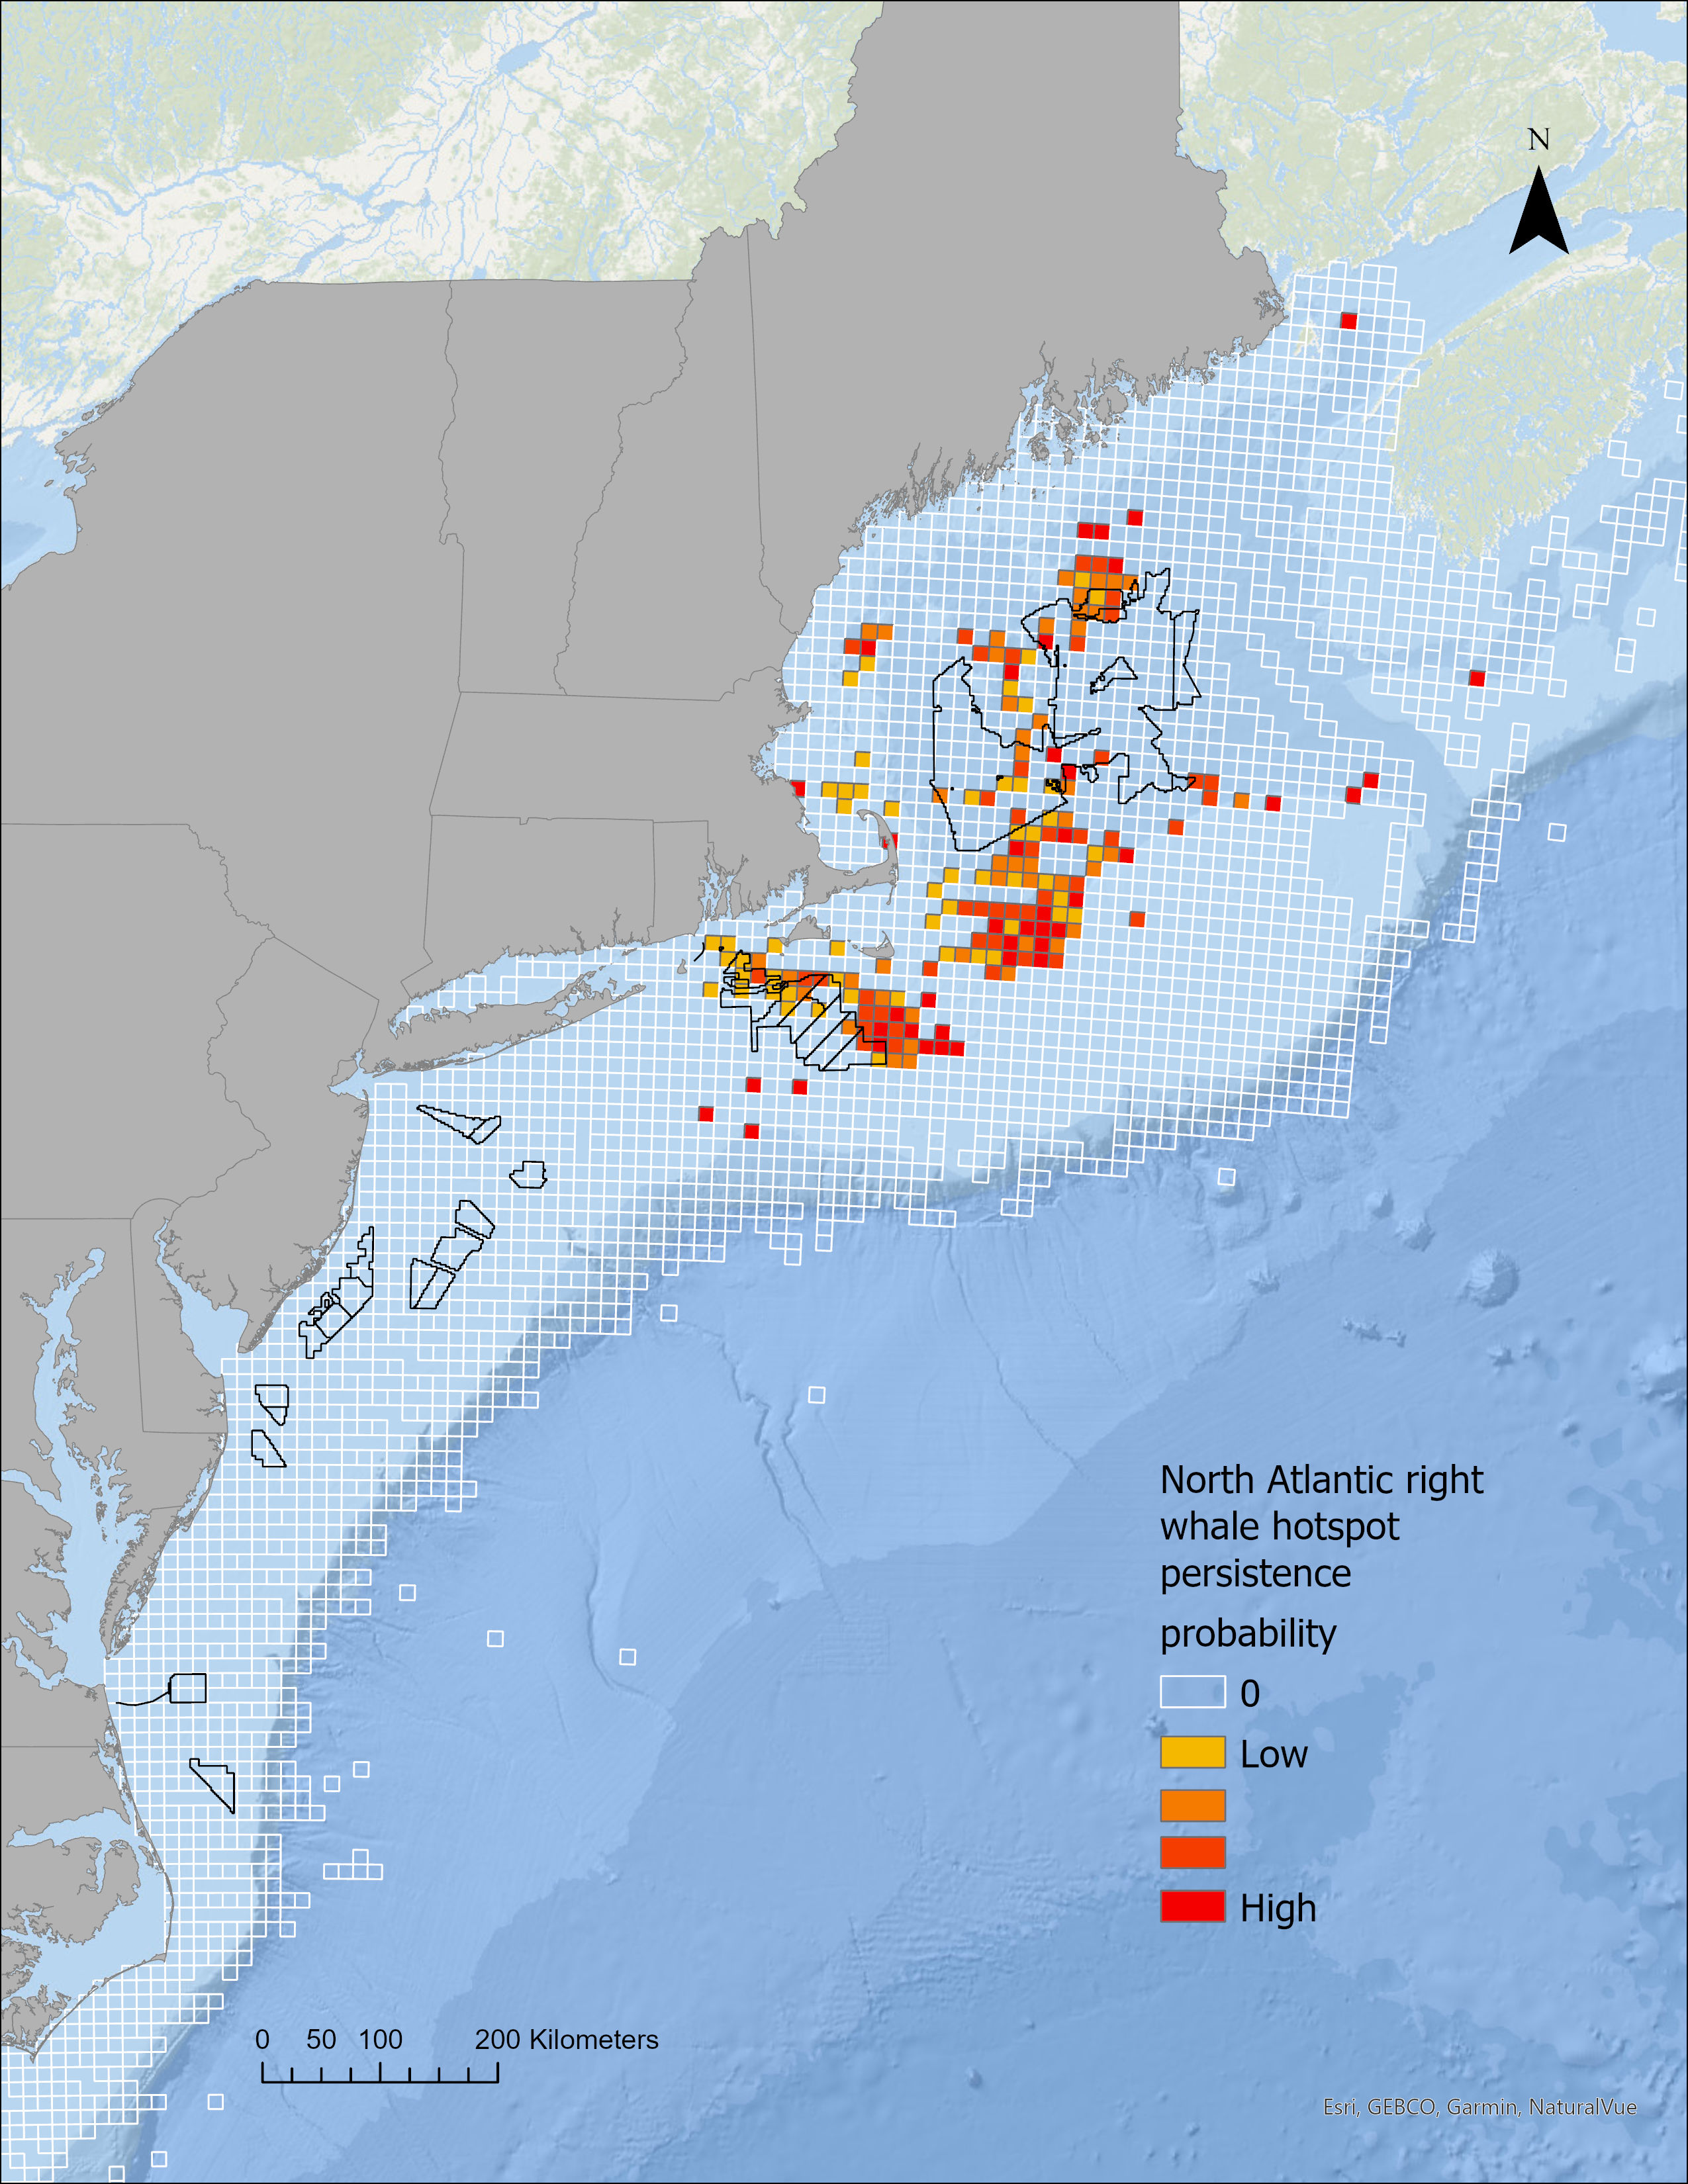
\includegraphics[width=0.55\linewidth]{SOE-MAFMC-2024_files/figure-latex/whales-wind-1} 

}

\caption{Northern Right Whale persistent hotspots (red shading) and Wind Energy Areas (black outlines).}\label{fig:whales-wind}
\end{figure}

Scientific data collection surveys for ocean and ecosystem conditions, fish, and protected species will be altered, potentially increasing uncertainty for stock assessments and associated management decision making.

The increase of offshore wind development can have both positive (e.g., employment opportunities) and negative (e.g., space-use conflicts) effects. Continued increase in coastal development and gentrification pressure has resulted in loss of fishing infrastructure space within ports. Understanding these existing pressures can allow for avoiding and mitigating negative impacts to our shore support industry and communities dependent on fishing. Some of the communities with the highest fisheries revenue overlap with offshore wind development areas that are also vulnerable to gentrification pressure are Point Pleasant and Atlantic City, NJ, Ocean City, MD, and Beaufort, NC.

\hypertarget{highlights}{%
\subsubsection{2023 Highlights}\label{highlights}}

This new section is common to the Mid-Atlantic and New England reports. Multiple \href{https://noaa-edab.github.io/catalog/observation_synthesis.html}{anomalous conditions} and extreme events were observed in 2023 that could have brief local effects and/or widespread long-term ecosystem, fishery and management implications. This section intends to provide a record of these observations, the implications they may have for other ecosystem processes, and a reflection on how they fit into our understanding of the ecosystem. Many of these observations are being actively studied but should be noted and considered in future analyses and management decisions.

Globally, 2023 was the warmest year on record with record high sea surface temperatures in the North Atlantic. In contrast, Northeast U.S. shelf surface temperatures were more variable, with near record highs in winter and near average conditions in other seasons.

\hypertarget{regionalcoastal-phenomena}{%
\paragraph{Regional/Coastal phenomena}\label{regionalcoastal-phenomena}}

There was a documented \href{https://noaa-edab.github.io/catalog/observation_synthesis.html}{die-off of scallops} in the Mid-Atlantic Elephant Trunk regions between the 2022 and 2023 surveys. In 2022, Elephant Trunk experienced \href{https://noaa-edab.github.io/catalog/thermal_habitat_persistence.html}{stressful temperatures} for scallops (17 - 19 ℃) for an average of 30 days (Fig. \ref{fig:elephantrunk}), but ongoing research is being conducted to identify contributing factors. A fish and shellfish mortality event was observed in coastal New Jersey linked to \href{https://noaa-edab.github.io/catalog/ocean_acidification.html}{hypoxia and ocean acidification} (Fig. \ref{fig:NJhypoxia}).

\begin{figure}

{\centering 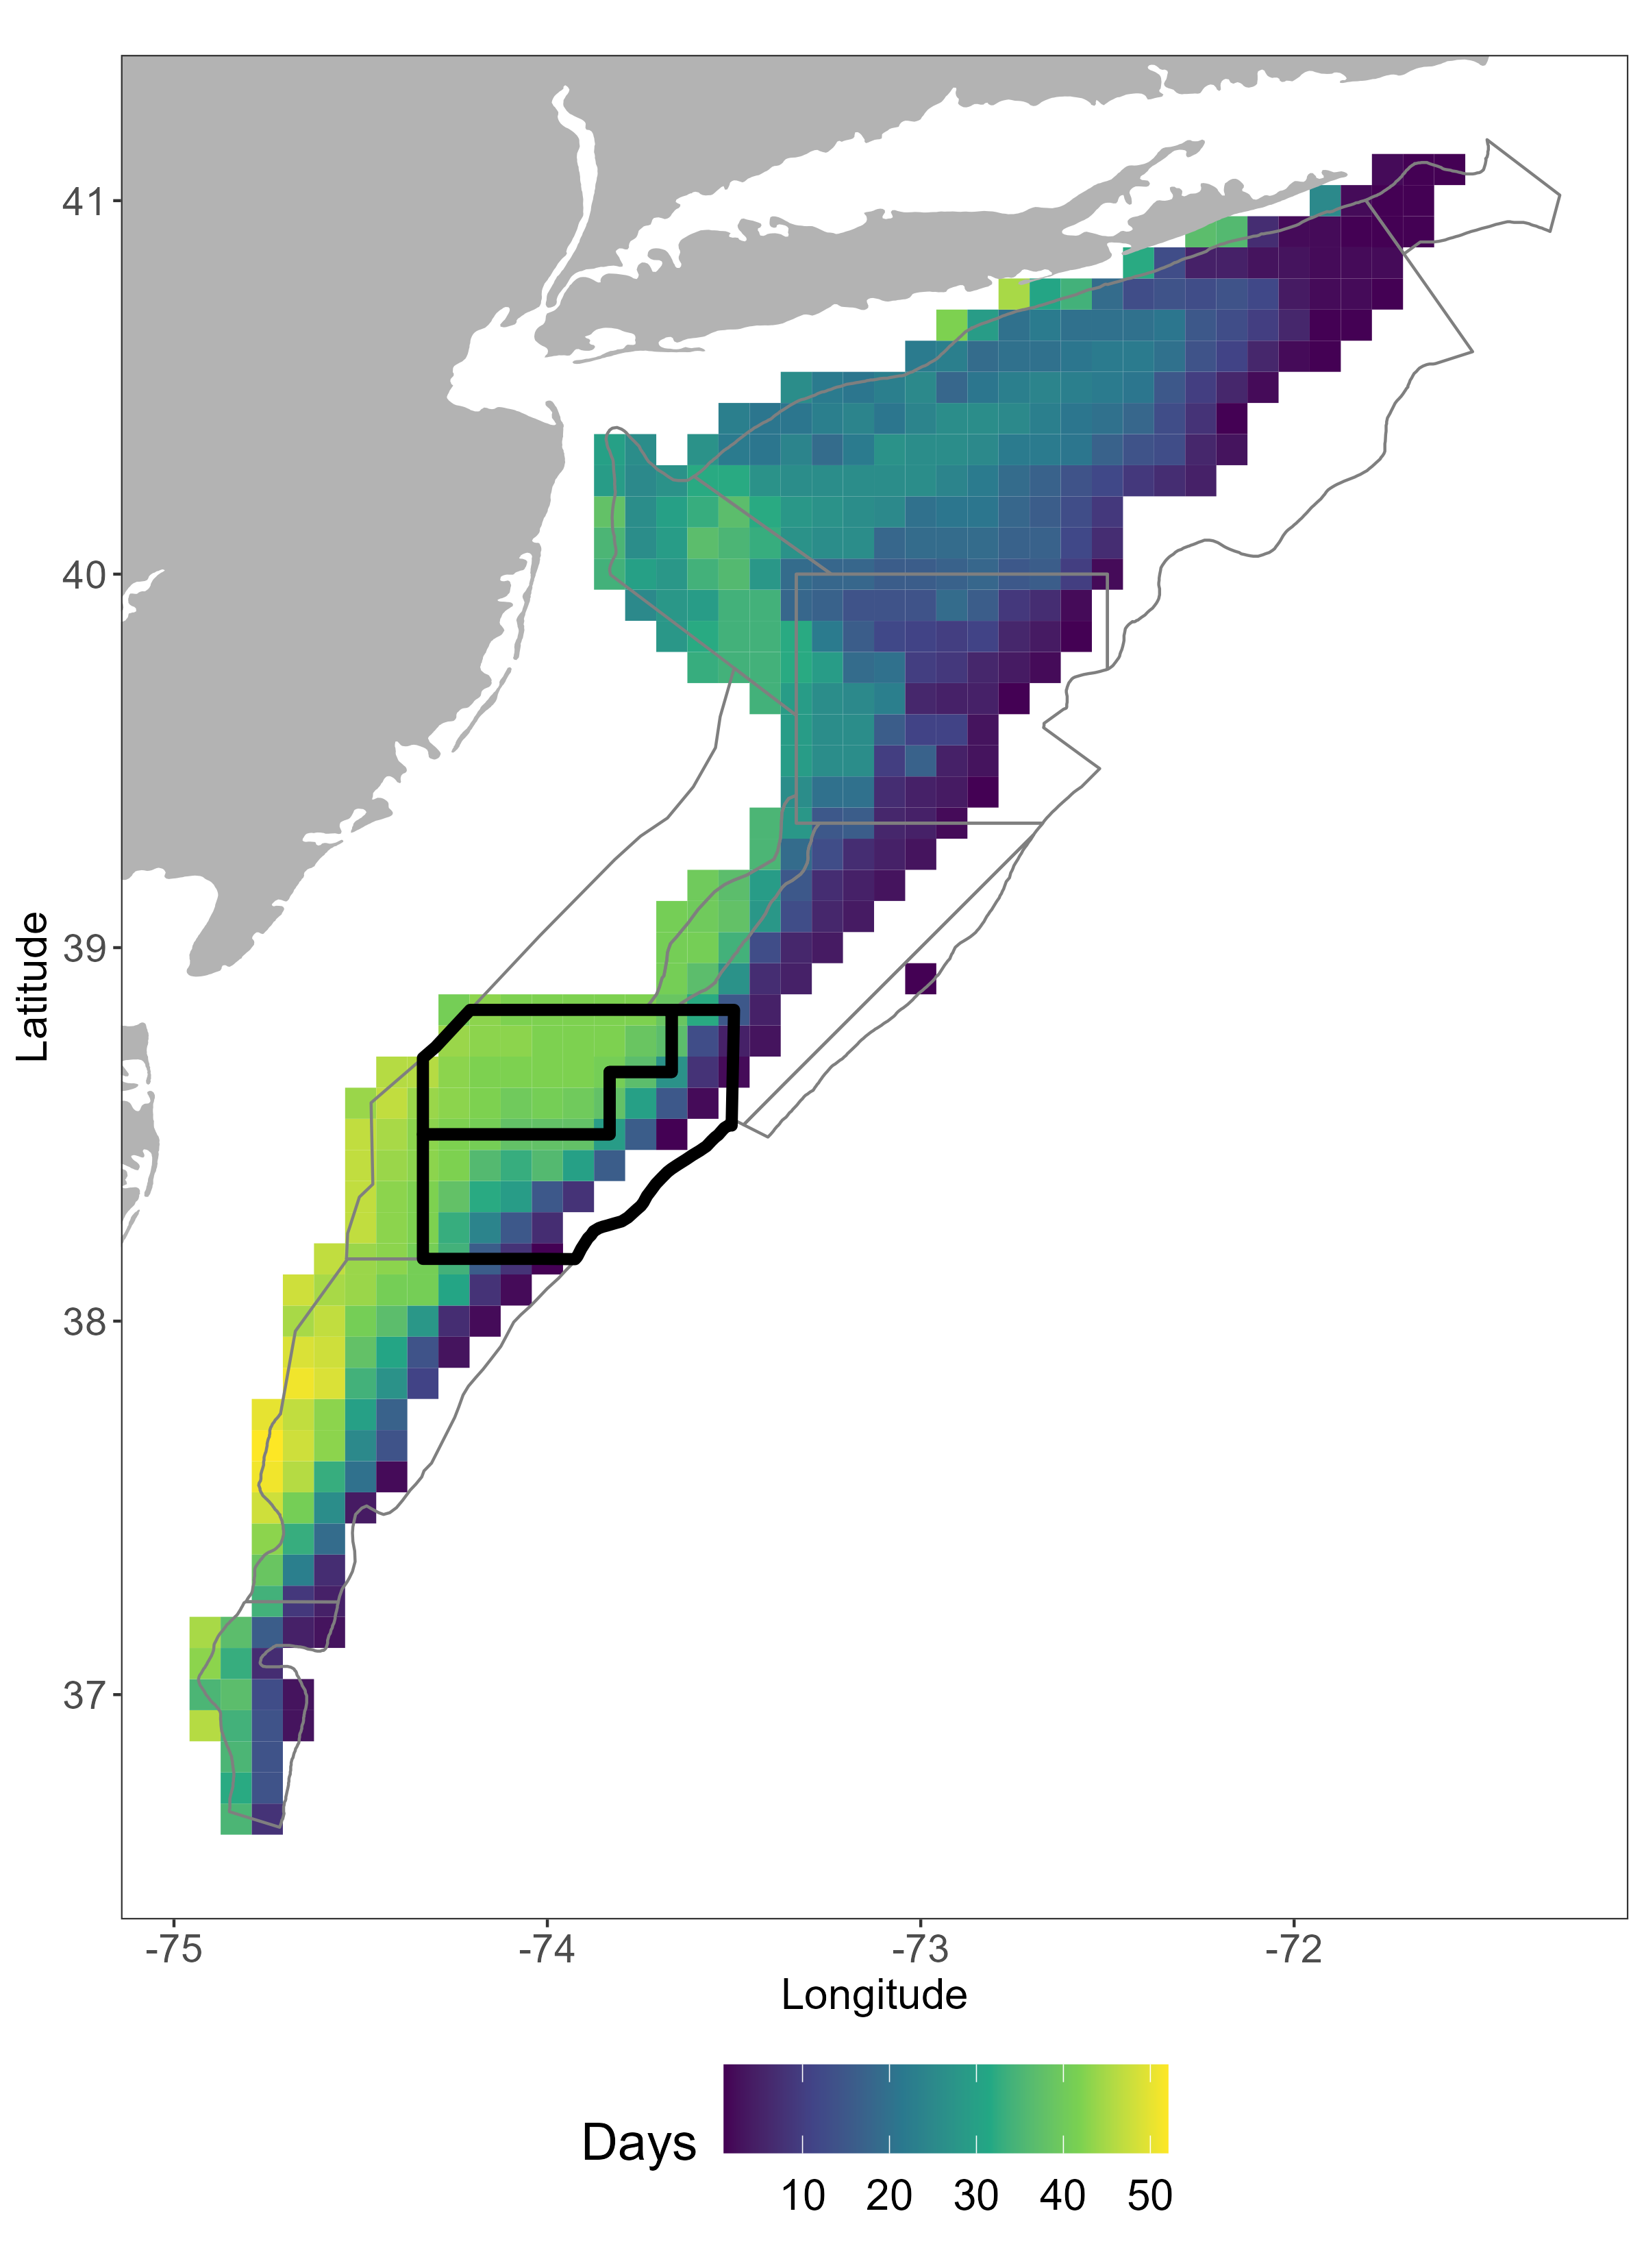
\includegraphics[width=0.5\linewidth]{SOE-MAFMC-2024_files/figure-latex/elephantrunk-1} 

}

\caption{The number of days where bottom temperature was between 17 and 19 °C in each GLORYS grid cell for 2022. The gray lines show the sea scallop estimation areas, with the Elephant Trunk region highlighted in black lines.}\label{fig:elephantrunk}
\end{figure}

\begin{figure}

{\centering 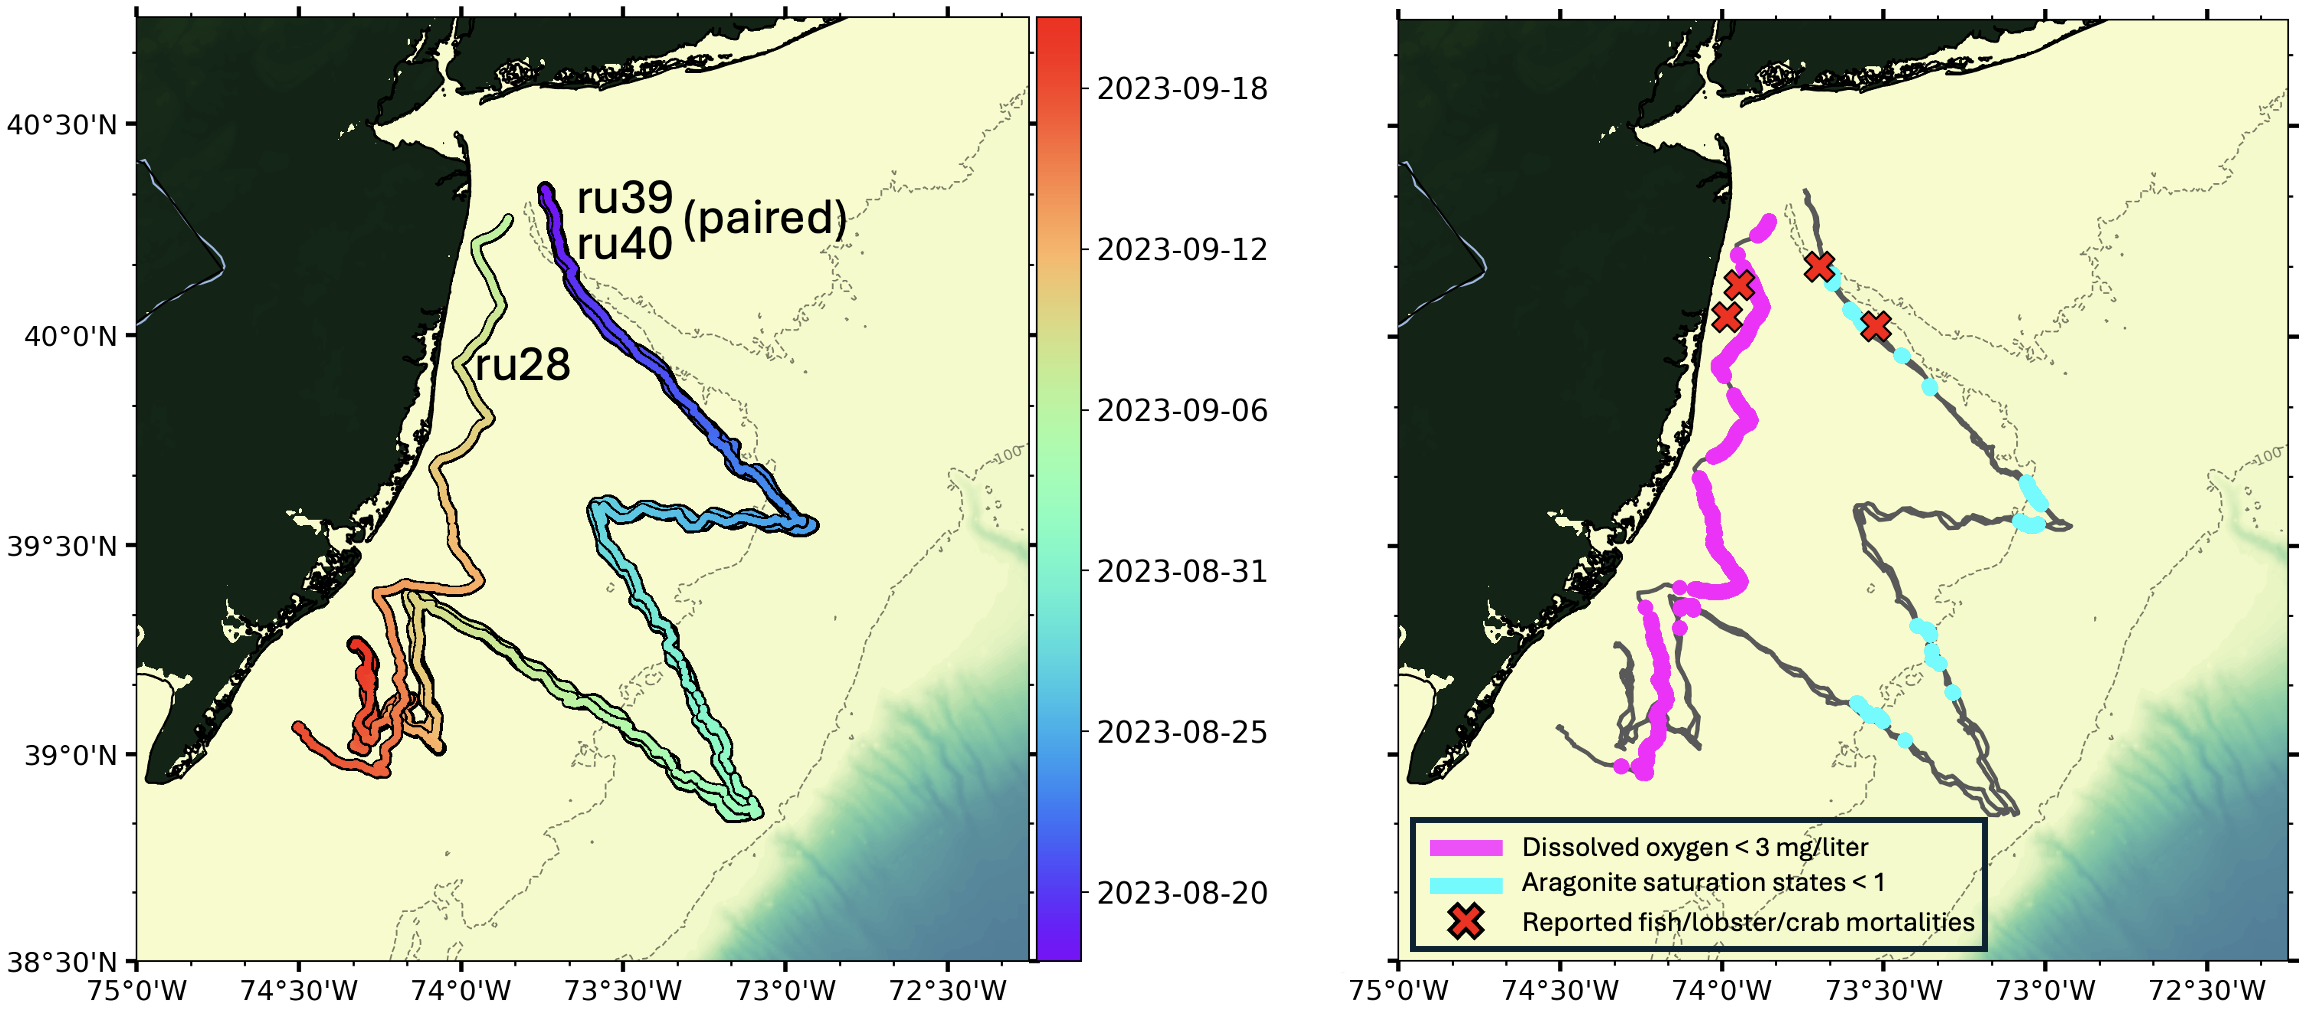
\includegraphics[width=0.5\linewidth]{SOE-MAFMC-2024_files/figure-latex/NJhypoxia-1} 

}

\caption{Mission tracks of three gliders (left) deployed off the coast of New Jersey in August and September of 2023. Locations of hypoxic levels of dissolved oxygen (magenta; < 3 mg/liter) and low aragonite saturation state (cyan; < 1) measured along the glider mission tracks and locations of reported fish, lobster, and/or crab mortalities (red X).}\label{fig:NJhypoxia}
\end{figure}

Summer \href{https://noaa-edab.github.io/catalog/bottom_temp_comp.html}{bottom temperatures} in the Gulf of Maine were the warmest on record (since 1959) resulting in the second largest \href{https://noaa-edab.github.io/catalog/heatwave_year.html}{bottom marine heatwave}. The heatwave started in February, peaked in May and likely continued beyond August (pending data update). \href{https://noaa-edab.github.io/catalog/thermal_habitat_persistence.html}{2023 bottom temperature} exceeded the 15 ℃ threshold for up to 59 days along the shelf break.

A wide-spread, long-duration \href{https://noaa-edab.github.io/catalog/observation_synthesis.html}{phytoplankton bloom} of the dinoflagellate \emph{Tripos muelleri} was observed in the GOM and generated chlorophyll concentrations up to ten times greater than average (a record high since 1998) from March to August (Figs. \ref{fig:chl-current-year}, \ref{fig:GOMbloom}). The bloom severely reduced water clarity, impacting harpoon fishing and likely affecting visual predators. Despite \emph{Tripos} being a similar size to typical large phytoplankton (diatoms), this extra production was not grazed nor did it sink to the bottom. The specific drivers of the bloom and implications to the food web are still under investigation.

\begin{figure}

{\centering \includegraphics{SOE-MAFMC-2024_files/figure-latex/chl-current-year-1} 

}

\caption{2023 median weekly chlorophyll concentrations (green line) with standard deviation 1998-2023 (gray shading).}\label{fig:chl-current-year}
\end{figure}

\begin{figure}

{\centering 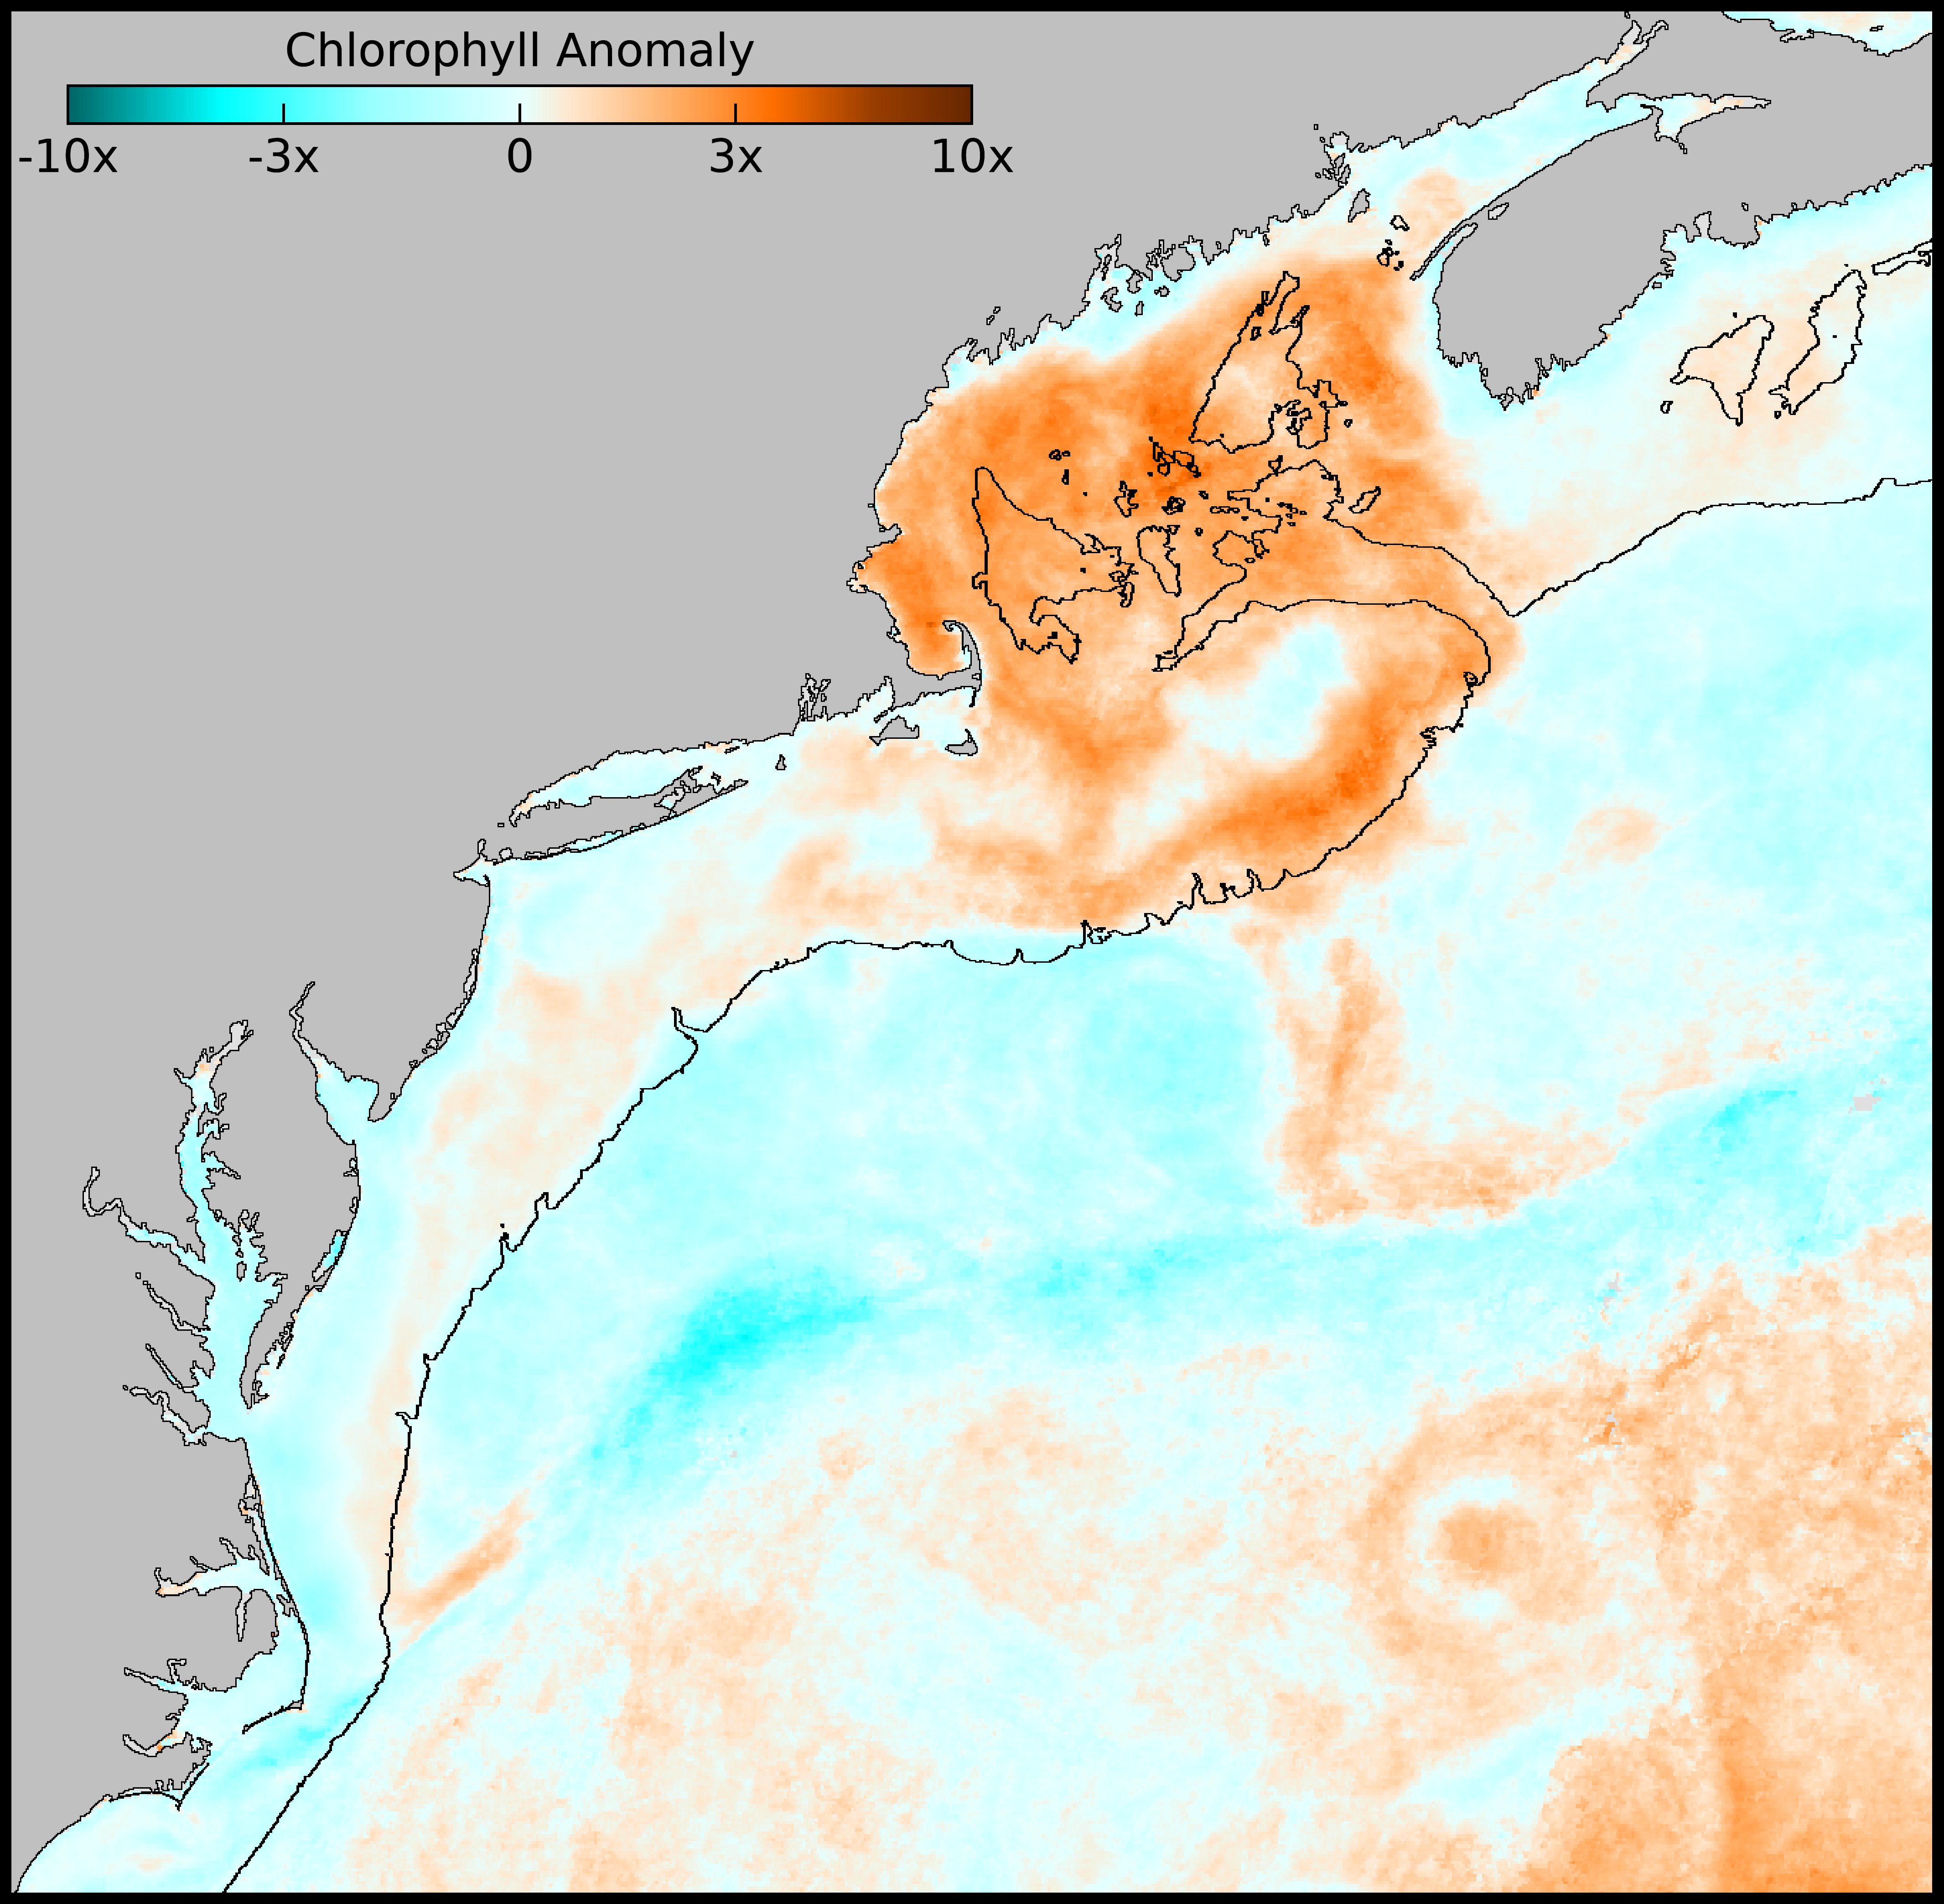
\includegraphics[width=0.5\linewidth]{SOE-MAFMC-2024_files/figure-latex/GOMbloom-1} 

}

\caption{June 2023 chlorophyll anomaly shown as the ratio of the June 2023 average compared to climatological (1998-2023) June average. The black line depicts the 100 m isobath.}\label{fig:GOMbloom}
\end{figure}

In Chesapeake Bay, \href{https://noaa-edab.github.io/catalog/ches_bay_synthesis.html}{hypoxia conditions} were the lowest on record (since 1995), creating more suitable habitat for multiple fin fish and benthic species. Cooler \href{https://noaa-edab.github.io/catalog/ches_bay_sst.html}{Chesapeake Bay water temperatures} paired with low hypoxia in the summer suggest conditions that season were favorable for striped bass. Cooler summer temperatures also support juvenile summer flounder growth. However, warmer winter and spring water temperatures in the Chesapeake Bay, along with other environmental factors (such as low flow), may have played a role in low production of juvenile striped bass in 2023. Higher-than-average \href{https://noaa-edab.github.io/catalog/ch_bay_sal.html}{salinity} across the Bay was likely driven by low precipitation and increased the area of available habitat for species such as croaker, spot, menhaden, and red drum, while restricting habitat area for invasive blue catfish.

\hypertarget{shelf-wide-phenomena}{%
\paragraph{Shelf-wide Phenomena}\label{shelf-wide-phenomena}}

The \href{https://noaa-edab.github.io/catalog/observation_synthesis.html}{Gulf Stream} was highly variable in 2023, with northward shifts intermittently throughout the year and a more notable prolonged shift north along the continental shelf break in the southern Mid-Atlantic in the fall (Fig. \ref{fig:gulfstream23}). This shift severely constricted the Slope Sea (the waters between the Gulf Stream and continental shelf), inhibited warm core ring formation and interactions, resulted in unusually warm and salty surface waters, and strong northeastward currents in the southern Mid-Atlantic. Intermittent warm waters like this can be threats to temperature sensitive species, especially species at the southern end of their range or are not mobile (e.g.~scallops), while also providing suitable habitat for more southern species.

\begin{figure}

{\centering 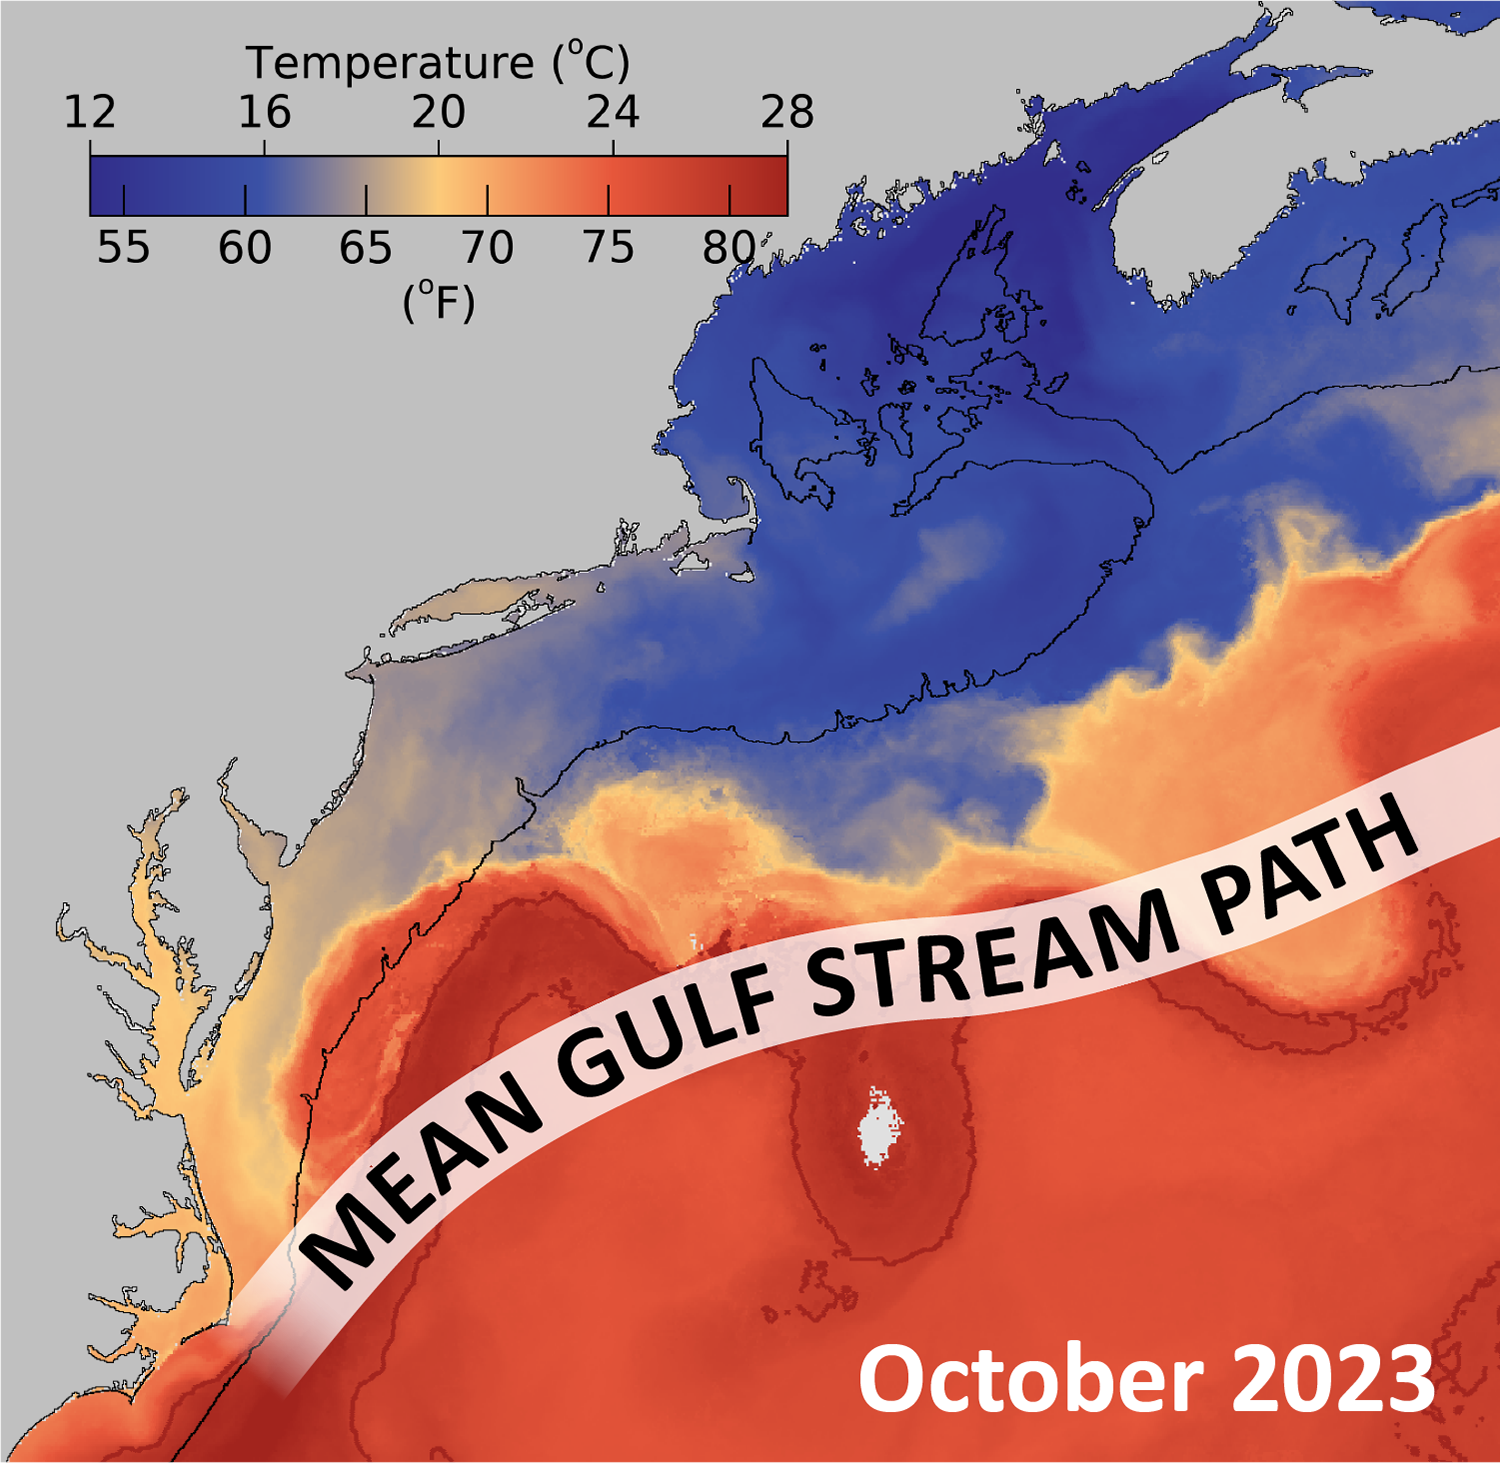
\includegraphics[width=0.5\linewidth]{SOE-MAFMC-2024_files/figure-latex/gulfstream23-1} 

}

\caption{October 8-14, 2023 sea surface temperature average derived from the Advanced Clear Sky Processor for Ocean (ACSPO) SST data. The black line depicts the 100 m isobath and the white line is the mean path of the Gulf Stream.}\label{fig:gulfstream23}
\end{figure}

While the total number of \href{https://noaa-edab.github.io/catalog/wcr.html}{warm core rings} in 2023 (18) was below the decadal average (31), there were a few notable events. A large early season ring pulled continental shelf water into the Slope Sea. Events like these can create biological hotspots, aggregating multiple species in small areas, increasing bycatch risks, and marine mammal shipstrike risks. In spring 2023, concentrations of North Atlantic right whales, humpback whales, basking sharks, and other large baleen whales were observed feeding near the edge of warm core rings near the shelf break.

Multiple fall 2023 tropical and coastal storms caused several flash flood events, above average coastal water levels, strong winds and high rainfall totals throughout the Northeast. These storms may be related to the shift from 2020-2022 La Niña conditions to strong El Niño conditions in late spring 2023. El Niño winters are associated with more frequent East Coast storms, which can result in increased risk of coastal flooding, increased freshwater runoff into the coastal ocean, and delayed spring transition from a well mixed water column to stratified. In estuaries, increased freshwater flow decreases salinity, reduces the amount of suitable habitat for juvenile marine fish, and is related to increased hypoxia (low oxygen). However, precipitation is not uniform throughout the Northeast U.S., and \href{https://noaa-edab.github.io/catalog/ch_bay_sal.html}{Chesapeake Bay 2023 conditions} did not align with El Nino expectations. The current El Niño is expected to weaken by spring 2024.

\hypertarget{contributors}{%
\section{Contributors}\label{contributors}}

\textbf{Editors} (NOAA NMFS Northeast Fisheries Science Center, NEFSC): Sarah Gaichas, Joseph Caracappa, Andy Beet, Brandon Beltz, Geret DePiper, Kimberly Hyde, Scott Large, Sean Lucey, Laurel Smith

\textbf{Contributors} (NEFSC unless otherwise noted): Kimberly Bastille, Aaron Beaver (Anchor QEA), Andy Beet, Brandon Beltz, Ruth Boettcher (Virginia Department of Game and Inland Fisheries), Mandy Bromilow and CJ Pellerin (NOAA Chesapeake Bay Office), Joseph Caracappa, Baoshan Chen (Stony Brook University), Doug Christel (GARFO), Patricia Clay, Lisa Colburn, Jennifer Cudney and Tobey Curtis (NMFS Atlantic HMS Management Division), Geret DePiper, Dan Dorfman (NOAA-NOS-NCCOS), Hubert du Pontavice, Emily Farr and Grace Roskar (NMFS Office of Habitat Conservation), Michael Fogarty, Paula Fratantoni, Kevin Friedland, Marjy Friedrichs (VIMS), Sarah Gaichas, Ben Galuardi (GAFRO), Avijit Gangopadhyay (School for Marine Science and Technology, University of Massachusetts Dartmouth), James Gartland (Virginia Institute of Marine Science), Lori Garzio (Rutgers University), Glen Gawarkiewicz (Woods Hole Oceanographic Institution), Sean Hardison, Dvora Hart, Kimberly Hyde, John Kocik, Steve Kress and Don Lyons (National Audubon Society's Seabird Restoration Program), Young-Oh Kwon and Zhuomin Chen (Woods Hole Oceanographic Institution), Andrew Lipsky, Sean Lucey, Chris Melrose, Shannon Meseck, Ryan Morse, Ray Mroch (SEFSC), Brandon Muffley (MAFMC), Kimberly Murray, David Moe Nelson (NCCOS), Janet Nye (University of North Carolina at Chapel Hill), Chris Orphanides, Richard Pace,Debi Palka, Tom Parham (Maryland DNR), Charles Perretti, Jeffrey Runge (U Maine), Grace Saba and Emily Slesinger (Rutgers University), Vincent Saba, Sarah Salois, Chris Schillaci (GARFO), Amy Schueller (SEFSC), Teresa Schwemmer (Stony Brook University), Dave Secor (CBL), Angela Silva, Adrienne Silver (UMass/SMAST), Laurel Smith, Talya tenBrink (GARFO), Abigail Tyrell, Bruce Vogt (NOAA Chesapeake Bay Office), Ron Vogel (University of Maryland Cooperative Institute for Satellite Earth System Studies and NOAA/NESDIS Center for Satellite Applications and Research), John Walden, Harvey Walsh, Changhua Weng, Dave Wilcox (VIMS), Timothy White (Environmental Studies Program, BOEM), Mark Wuenschel, Qian Zhang (U Maryland)

\hypertarget{document-orientation}{%
\section{Document Orientation}\label{document-orientation}}

The figure format is illustrated in Fig \ref{fig:docformat}a. Trend lines are shown when slope is significantly different from 0 at the p \textless{} 0.05 level. An orange line signifies an overall positive trend, and purple signifies a negative trend. To minimize bias introduced by small sample size, no trend is fit for \textless{} 30 year time series. Dashed lines represent mean values of time series unless the indicator is an anomaly, in which case the dashed line is equal to 0. Shaded regions indicate the past ten years. If there are no new data for 2022, the shaded region will still cover this time period. The spatial scale of indicators is either coastwide, Mid-Atlantic states (New York, New Jersey, Delaware, Maryland, Virginia, North Carolina), or at the Mid-Atlantic Bight (MAB) Ecosystem Production Unit (EPU, Fig. \ref{fig:docformat}b) level.

\begin{figure}

{\centering \includegraphics{SOE-MAFMC-2024_files/figure-latex/docformat-1} 

}

\caption{Document orientation. a. Key to figures. b.The Northeast Large Marine Ecosystem.}\label{fig:docformat}
\end{figure}

Fish and invertebrates are aggregated into similar feeding categories (Table \ref{tab:species-groupings}) to evaluate ecosystem level trends in predators and prey.

\global\setlength{\Oldarrayrulewidth}{\arrayrulewidth}

\global\setlength{\Oldtabcolsep}{\tabcolsep}

\setlength{\tabcolsep}{0pt}

\renewcommand*{\arraystretch}{1.5}



\providecommand{\ascline}[3]{\noalign{\global\arrayrulewidth #1}\arrayrulecolor[HTML]{#2}\cline{#3}}

\begin{longtable}[c]{|p{1.00in}|p{1.00in}|p{1.00in}|p{1.00in}|p{3.00in}}

\caption{Feeding\ guilds\ and\ management\ bodies.}\label{tab:species-groupings}\\

\ascline{1.5pt}{666666}{1-5}

\multicolumn{1}{>{\raggedright}m{\dimexpr 1in+0\tabcolsep}}{\textcolor[HTML]{000000}{\fontsize{8}{8}\selectfont{Guild}}} & \multicolumn{1}{>{\raggedright}m{\dimexpr 1in+0\tabcolsep}}{\textcolor[HTML]{000000}{\fontsize{8}{8}\selectfont{MAFMC}}} & \multicolumn{1}{>{\raggedright}m{\dimexpr 1in+0\tabcolsep}}{\textcolor[HTML]{000000}{\fontsize{8}{8}\selectfont{Joint}}} & \multicolumn{1}{>{\raggedright}m{\dimexpr 1in+0\tabcolsep}}{\textcolor[HTML]{000000}{\fontsize{8}{8}\selectfont{NEFMC}}} & \multicolumn{1}{>{\raggedright}m{\dimexpr 3in+0\tabcolsep}}{\textcolor[HTML]{000000}{\fontsize{8}{8}\selectfont{State\ or\ Other}}} \\

\ascline{1.5pt}{666666}{1-5}\endfirsthead \caption[]{Feeding\ guilds\ and\ management\ bodies.}\label{tab:species-groupings}\\

\ascline{1.5pt}{666666}{1-5}

\multicolumn{1}{>{\raggedright}m{\dimexpr 1in+0\tabcolsep}}{\textcolor[HTML]{000000}{\fontsize{8}{8}\selectfont{Guild}}} & \multicolumn{1}{>{\raggedright}m{\dimexpr 1in+0\tabcolsep}}{\textcolor[HTML]{000000}{\fontsize{8}{8}\selectfont{MAFMC}}} & \multicolumn{1}{>{\raggedright}m{\dimexpr 1in+0\tabcolsep}}{\textcolor[HTML]{000000}{\fontsize{8}{8}\selectfont{Joint}}} & \multicolumn{1}{>{\raggedright}m{\dimexpr 1in+0\tabcolsep}}{\textcolor[HTML]{000000}{\fontsize{8}{8}\selectfont{NEFMC}}} & \multicolumn{1}{>{\raggedright}m{\dimexpr 3in+0\tabcolsep}}{\textcolor[HTML]{000000}{\fontsize{8}{8}\selectfont{State\ or\ Other}}} \\

\ascline{1.5pt}{666666}{1-5}\endhead



\multicolumn{1}{>{\raggedright}m{\dimexpr 1in+0\tabcolsep}}{\textcolor[HTML]{000000}{\fontsize{8}{8}\selectfont{Apex\ Predator}}} & \multicolumn{1}{>{\raggedright}m{\dimexpr 1in+0\tabcolsep}}{\textcolor[HTML]{000000}{\fontsize{8}{8}\selectfont{}}} & \multicolumn{1}{>{\raggedright}m{\dimexpr 1in+0\tabcolsep}}{\textcolor[HTML]{000000}{\fontsize{8}{8}\selectfont{}}} & \multicolumn{1}{>{\raggedright}m{\dimexpr 1in+0\tabcolsep}}{\textcolor[HTML]{000000}{\fontsize{8}{8}\selectfont{}}} & \multicolumn{1}{>{\raggedright}m{\dimexpr 3in+0\tabcolsep}}{\textcolor[HTML]{000000}{\fontsize{8}{8}\selectfont{shark\ uncl,\ swordfish,\ yellowfin\ tuna,\ bluefin\ tuna}}} \\





\multicolumn{1}{>{\raggedright}m{\dimexpr 1in+0\tabcolsep}}{\textcolor[HTML]{000000}{\fontsize{8}{8}\selectfont{Piscivore}}} & \multicolumn{1}{>{\raggedright}m{\dimexpr 1in+0\tabcolsep}}{\textcolor[HTML]{000000}{\fontsize{8}{8}\selectfont{summer\ flounder,\ bluefish,\ northern\ shortfin\ squid,\ longfin\ squid}}} & \multicolumn{1}{>{\raggedright}m{\dimexpr 1in+0\tabcolsep}}{\textcolor[HTML]{000000}{\fontsize{8}{8}\selectfont{spiny\ dogfish,\ goosefish}}} & \multicolumn{1}{>{\raggedright}m{\dimexpr 1in+0\tabcolsep}}{\textcolor[HTML]{000000}{\fontsize{8}{8}\selectfont{winter\ skate,\ clearnose\ skate,\ thorny\ skate,\ offshore\ hake,\ silver\ hake,\ atlantic\ cod,\ pollock,\ white\ hake,\ red\ hake,\ atlantic\ halibut,\ acadian\ redfish}}} & \multicolumn{1}{>{\raggedright}m{\dimexpr 3in+0\tabcolsep}}{\textcolor[HTML]{000000}{\fontsize{8}{8}\selectfont{sea\ lamprey,\ sandbar\ shark,\ atlantic\ angel\ shark,\ atlantic\ torpedo,\ conger\ eel,\ spotted\ hake,\ cusk,\ fourspot\ flounder,\ windowpane,\ john\ dory,\ atlantic\ cutlassfish,\ blue\ runner,\ striped\ bass,\ weakfish,\ sea\ raven,\ northern\ stargazer,\ banded\ rudderfish,\ atlantic\ sharpnose\ shark,\ inshore\ lizardfish,\ atlantic\ brief\ squid,\ northern\ sennet,\ king\ mackerel,\ spanish\ mackerel}}} \\





\multicolumn{1}{>{\raggedright}m{\dimexpr 1in+0\tabcolsep}}{\textcolor[HTML]{000000}{\fontsize{8}{8}\selectfont{Planktivore}}} & \multicolumn{1}{>{\raggedright}m{\dimexpr 1in+0\tabcolsep}}{\textcolor[HTML]{000000}{\fontsize{8}{8}\selectfont{atlantic\ mackerel,\ butterfish}}} & \multicolumn{1}{>{\raggedright}m{\dimexpr 1in+0\tabcolsep}}{\textcolor[HTML]{000000}{\fontsize{8}{8}\selectfont{}}} & \multicolumn{1}{>{\raggedright}m{\dimexpr 1in+0\tabcolsep}}{\textcolor[HTML]{000000}{\fontsize{8}{8}\selectfont{atlantic\ herring}}} & \multicolumn{1}{>{\raggedright}m{\dimexpr 3in+0\tabcolsep}}{\textcolor[HTML]{000000}{\fontsize{8}{8}\selectfont{harvestfishes,\ smelts,\ round\ herring,\ alewife,\ blueback\ herring,\ american\ shad,\ menhaden,\ bay\ anchovy,\ striped\ anchovy,\ rainbow\ smelt,\ atlantic\ argentine,\ slender\ snipe\ eel,\ atlantic\ silverside,\ northern\ pipefish,\ chub\ mackerel,\ atlantic\ moonfish,\ lookdown,\ blackbelly\ rosefish,\ lumpfish,\ northern\ sand\ lance,\ atlantic\ saury,\ mackerel\ scad,\ bigeye\ scad,\ round\ scad,\ rough\ scad,\ silver\ rag,\ weitzmans\ pearlsides,\ atlantic\ soft\ pout,\ sevenspine\ bay\ shrimp,\ pink\ glass\ shrimp,\ polar\ lebbeid,\ friendly\ blade\ shrimp,\ bristled\ longbeak,\ aesop\ shrimp,\ norwegian\ shrimp,\ northern\ shrimp,\ brown\ rock\ shrimp,\ atlantic\ thread\ herring,\ spanish\ sardine,\ atlantic\ bumper,\ harvestfish,\ striated\ argentine,\ silver\ anchovy}}} \\





\multicolumn{1}{>{\raggedright}m{\dimexpr 1in+0\tabcolsep}}{\textcolor[HTML]{000000}{\fontsize{8}{8}\selectfont{Benthivore}}} & \multicolumn{1}{>{\raggedright}m{\dimexpr 1in+0\tabcolsep}}{\textcolor[HTML]{000000}{\fontsize{8}{8}\selectfont{black\ sea\ bass,\ scup,\ tilefish}}} & \multicolumn{1}{>{\raggedright}m{\dimexpr 1in+0\tabcolsep}}{\textcolor[HTML]{000000}{\fontsize{8}{8}\selectfont{}}} & \multicolumn{1}{>{\raggedright}m{\dimexpr 1in+0\tabcolsep}}{\textcolor[HTML]{000000}{\fontsize{8}{8}\selectfont{barndoor\ skate,\ rosette\ skate,\ little\ skate,\ smooth\ skate,\ haddock,\ american\ plaice,\ yellowtail\ flounder,\ winter\ flounder,\ witch\ flounder,\ ocean\ pout,\ crab,red\ deepsea}}} & \multicolumn{1}{>{\raggedright}m{\dimexpr 3in+0\tabcolsep}}{\textcolor[HTML]{000000}{\fontsize{8}{8}\selectfont{crab,unc,\ hagfish,\ porgy,red,\ sea\ bass,nk,\ atlantic\ hagfish,\ roughtail\ stingray,\ smooth\ dogfish,\ chain\ dogfish,\ bluntnose\ stingray,\ bullnose\ ray,\ southern\ stingray,\ longfin\ hake,\ fourbeard\ rockling,\ marlin-spike,\ gulf\ stream\ flounder,\ longspine\ snipefish,\ blackmouth\ bass,\ threespine\ stickleback,\ smallmouth\ flounder,\ hogchoker,\ bigeye,\ atlantic\ croaker,\ pigfish,\ northern\ kingfish,\ silver\ perch,\ spot,\ deepbody\ boarfish,\ sculpin\ uncl,\ moustache\ sculpin,\ longhorn\ sculpin,\ alligatorfish,\ grubby,\ atlantic\ seasnail,\ northern\ searobin,\ striped\ searobin,\ armored\ searobin,\ cunner,\ tautog,\ snakeblenny,\ daubed\ shanny,\ radiated\ shanny,\ red\ goatfish,\ striped\ cusk-eel,\ wolf\ eelpout,\ wrymouth,\ atlantic\ wolffish,\ fawn\ cusk-eel,\ northern\ puffer,\ striped\ burrfish,\ planehead\ filefish,\ gray\ triggerfish,\ shortnose\ greeneye,\ beardfish,\ cownose\ ray,\ american\ lobster,\ cancer\ crab\ uncl,\ jonah\ crab,\ atlantic\ rock\ crab,\ blue\ crab,\ spider\ crab\ uncl,\ horseshoe\ crab,\ coarsehand\ lady\ crab,\ lady\ crab,\ northern\ stone\ crab,\ snow\ crab,\ spiny\ butterfly\ ray,\ smooth\ butterfly\ ray,\ snakefish,\ atlantic\ midshipman,\ bank\ cusk-eel,\ red\ cornetfish,\ squid\ cuttlefish\ and\ octopod\ uncl,\ spoonarm\ octopus,\ bank\ sea\ bass,\ rock\ sea\ bass,\ sand\ perch,\ cobia,\ crevalle\ jack,\ vermilion\ snapper,\ tomtate,\ jolthead\ porgy,\ saucereye\ porgy,\ whitebone\ porgy,\ knobbed\ porgy,\ sheepshead\ porgy,\ littlehead\ porgy,\ silver\ porgy,\ pinfish,\ red\ porgy,\ porgy\ and\ pinfish\ uncl,\ banded\ drum,\ southern\ kingfish,\ atlantic\ spadefish,\ leopard\ searobin,\ dusky\ flounder,\ triggerfish\ filefish\ uncl,\ blackcheek\ tonguefish,\ orange\ filefish,\ queen\ triggerfish,\ ocean\ triggerfish}}} \\





\multicolumn{1}{>{\raggedright}m{\dimexpr 1in+0\tabcolsep}}{\textcolor[HTML]{000000}{\fontsize{8}{8}\selectfont{Benthos}}} & \multicolumn{1}{>{\raggedright}m{\dimexpr 1in+0\tabcolsep}}{\textcolor[HTML]{000000}{\fontsize{8}{8}\selectfont{atlantic\ surfclam,\ ocean\ quahog}}} & \multicolumn{1}{>{\raggedright}m{\dimexpr 1in+0\tabcolsep}}{\textcolor[HTML]{000000}{\fontsize{8}{8}\selectfont{}}} & \multicolumn{1}{>{\raggedright}m{\dimexpr 1in+0\tabcolsep}}{\textcolor[HTML]{000000}{\fontsize{8}{8}\selectfont{sea\ scallop}}} & \multicolumn{1}{>{\raggedright}m{\dimexpr 3in+0\tabcolsep}}{\textcolor[HTML]{000000}{\fontsize{8}{8}\selectfont{sea\ cucumber,\ sea\ urchins,\ snails(conchs),\ sea\ urchin\ and\ sand\ dollar\ uncl,\ channeled\ whelk,\ blue\ mussel}}} \\

\ascline{1.5pt}{666666}{1-5}



\end{longtable}



\arrayrulecolor[HTML]{000000}

\global\setlength{\arrayrulewidth}{\Oldarrayrulewidth}

\global\setlength{\tabcolsep}{\Oldtabcolsep}

\renewcommand*{\arraystretch}{1}

\end{document}
